% ****** Start of file apssamp.tex ******
%
%   This file is part of the APS files in the REVTeX 4.1 distribution.
%   Version 4.1r of REVTeX, August 2010
%
%   Copyright (c) 2009, 2010 The American Physical Society.
%
%   See the REVTeX 4 README file for restrictions and more information.
%
% TeX'ing this file requires that you have AMS-LaTeX 2.0 installed
% as well as the rest of the prerequisites for REVTeX 4.1
%
% See the REVTeX 4 README file
% It also requires running BibTeX. The commands are as follows:
%
%  1)  latex apssamp.tex
%  2)  bibtex apssamp
%  3)  latex apssamp.tex
%  4)  latex apssamp.tex
%%
\documentclass[%
reprint,
%superscriptaddress,
%groupedaddress,
%unsortedaddress,
%runinaddress,
%frontmatterverbose,
% preprint,
%showpacs,preprintnumbers,
%nofootinbib,
%nobibnotes,
%bibnotes,
 amsmath,amssymb,
 aps,
 % pra,
prl,
%rmp,
%prstab,
%prstper,
%floatfix,
]{revtex4-1}

\usepackage{soul}
\usepackage{color}

\newcommand{\hlcyan}[1]{{\sethlcolor{cyan}\hl{#1}}}
\newcommand{\hlred}[1]{{\sethlcolor{red}\hl{#1}}}

\usepackage{graphicx}% Include figure files
\usepackage{dcolumn}% Align table columns on decimal point
\usepackage{bm}% bold math
\usepackage{hyperref}% add hypertext capabilities
%\usepackage[mathlines]{lineno}% Enable numbering of text and display math
%\linenumbers\relax % Commence numbering lines

%\usepackage[showframe,%Uncomment any one of the following lines to test
%%scale=0.7, marginratio={1:1, 2:3}, ignoreall,% default settings
%%text={7in,10in},centering,
%%margin=1.5in,
%%total={6.5in,8.75in}, top=1.2in, left=0.9in, includefoot,
%%height=10in,a5paper,hmargin={3cm,0.8in},
%]{geometry}
%

\usepackage{xcolor}
\newcommand{\DP}[1]{\noindent \color{cyan} (DP: #1)\normalcolor}
\newcommand{\AZ}[1]{\noindent \color{purple} (AZ: #1)\normalcolor}
\newcommand{\add}[1]{\noindent \color{blue} #1 \normalcolor}
\newcommand{\del}[1]{\noindent \color{red} \st{#1}\normalcolor}
\newcommand{\AM}[1]{\noindent \color{magenta} (AA: #1)\normalcolor}
\def\red{\textcolor{red}}
%
\def\blue{\textcolor{blue}}

\begin{document}
%
\preprint{APS/123-QED}

\title{Temporal Evolution of Erosion in Pore-Networks:\\ From Homogenization to Instability} 
% Force line breaks with \\
% \thanks{A footnote to the article title}%

\author{Ahmad Zareei}
\thanks{A.Z. and D.P. contributed equally.}
\affiliation{School of Engineering and Applied Sciences, Harvard University, Cambridge, MA, 02148}%\altaffiliation[]{SEAS, Pierce Hall}%Lines break automatically or can be forced with 
\author{Deng Pan}%
\thanks{A.Z. and D.P. contributed equally.}
\affiliation{School of Engineering and Applied Sciences, Harvard University, Cambridge, MA, 02148}%\altaffiliation[]{SEAS, Pierce Hall}%Lines break automatically or can be forced with
\author{Ariel Amir}%
\email{arielamir@seas.harvard.edu}
\affiliation{School of Engineering and Applied Sciences, Harvard University, Cambridge, MA, 02148}%\altaffiliation[]{SEAS, Pierce Hall}%Lines break  automatically or can be forced with
% need to figure out how to reference dagger

% \author{}
% \altaffiliation[]{SEAS, Pierce Hall}%Lines break automatically or can be forced with \\
% \author{}%
%  \email{}
% \affiliation{% SEAS, Pierce Hall, Harvard University}%

% \collaboration{MUSO Collaboration}%\noaffiliation

\date{\today}% It is always \today, today,
             %  but any date may be explicitly specified

\begin{abstract}
We study the dynamics of flow-networks in porous media using a two/three dimensional
pore-network model. We consider a class of erosion dynamics
for a single phase flow with no deposition, chemical reactions, or topology changes assuming a constitutive law depending on flow rate, local velocities, or shear stress at the walls. We show that depending on the erosion law, the flow may become uniform and homogenized or become unstable and develop channels. By defining an order parameter capturing these different behaviors we show that a phase transition occurs depending on the erosion dynamics. Using a simple model, we identify quantitative criteria to distinguish these regimes and {correctly predict the fate of the network, and discuss the experimental relevance of our result. }
%
% Lastly, we show that the initial stages of pores clogging show analogous behaviors which depends on the clogging dynamics.

% Lastly, we show that pores clogging at the initial stages show analogous behaviors depending on clogging dynamics. % , however, due to the pore throat blockages and changes in the network connections the evolution diverges from its initial trend.

% \begin{description}
% \item[Usage] Secondary publications and information retrieval purposes.
% \item[PACS numbers] May be entered using the \verb+\pacs{#1}+ command.
% \item[Structure] You may use the \texttt{description} environment to structure your abstract; use the optional argument of the \verb+\item+ command to give the category of each item.
% \end{description}
\end{abstract}

% 


% \pacs{Valid PACS appear here}% PACS, the Physics and Astronomy
                             % Classification Scheme.
%\keywords{Suggested keywords}%Use showkeys class option if keyword
                              %display desired
\maketitle
%%%%%%%%%%%%%%%%%%%%%%%%%%%%%%%%%%%%%%%%%%
%%%%%%%%% \tableofcontents %%%%%%%%%%%%%%%
%%%%%%%%%%%%%%%%%%%%%%%%%%%%%%%%%%%%%%%%%%
%%%%%%%%%% \section{Introduction} 
%%%%%%%%%%%%%%%%%%%%%%%%%%%%%%%%%%%%%%%%%%
%%%%% The fluids %%%%%%%%%%%%%%%%%%%%%%%%%
%%%%%%%%%%%%%%%%%%%%%%%%%%%%%%%%%%%%%%%%%%

Fluid flow through a porous medium undergoing a dynamical change in its network of micro-structure is ubiquitous in nature~\cite{marbach2016pruning,alim2013random,tero2010rules,heaton2010growth} as well as in numerous environmental~\cite{schlesinger1999carbon,winkler1979pore,batzle1992seismic,cohen2015mechanisms} and industrial applications~\cite{duduta2011semi,sun2019hierarchical,smith2017multiphase,ferguson2012nonequilibrium}.
The disordered pore structure of a porous medium results in heterogeneously distributed fluid flow between the pores.
The boundaries of the pore structure can change dynamically either through erosion or deposition/sedimentation of material. Such heterogeneous changes of the solid structure affect the pore-level fluid flow which in turn affects the dynamical changes to the pore structure. This feedback mechanism along with the initial heterogeneous fluid flow makes it difficult to understand and predict the porous media behavior. Nonetheless, an understanding of the dynamical change is essential to improve any of the porous media applications where the pore network changes over time, including groundwater remediation and precipitation of minerals in rocks~\cite{rad2013pore}, biofilm growth in water filtration, and protective filters \cite{herzig1970flow,tien1979advances,jaisi2008transport,carrel2018biofilms,seymour2004anomalous}, as well as enhanced oil recovery with polymer flooding \cite{lake2014fundamentals,parsa2020origin}, or water-driven erosion \cite{schorghofer2004spontaneous,mahadevan2012flow}. 



%%%%%%%%%%%%%%%%%%%%%%%%%%%%%%%%%%%%%%%%%%%5
% \section{Methods \& Results}
%%%%%%%%%%%%%%%%%%%%%%%%%%%%%%%%%%%%%%%%%%%%5
\begin{figure}[h]
    % \centering
    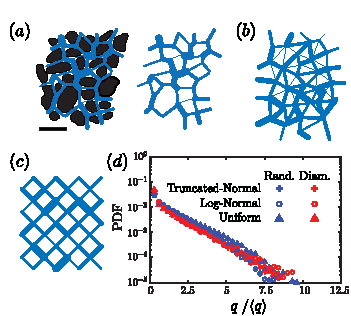
\includegraphics[width = 0.45\textwidth]{Fig1.pdf}
    % \caption{(a) Cross section of a porous sandstone sample obtained using  computerized tomography~\cite{akanji2010finite}. The scale in the bottom left shows $1$mm. The network of pores and throats is highlighted in blue. In the network model, the pores are represented with nodes and the throats between pores are approximated with tubes connecting the pores together. (b) Schematic of a topologically random network (i); and a structured diamond grid network (ii). The edge diameters in both networks are randomly distributed. The inset figure shows the conservation of mass at each node. (c) The universal probability distribution function (PDF) of fluid flux for a topologically random (in blue) or diamond network (red) with a highly disordered random network including uniform (triangles), log-normal (circles), and truncated normal (plus) distributions.}
    \caption{(a) Cross section of a porous sandstone sample obtained using  computerized tomography~\cite{akanji2010finite}. The scale in the bottom left shows $1$mm. The network of pores and throats is highlighted in blue. In the network model, the pores are represented with nodes and the throats between pores are approximated with tubes. (b) Schematic of a topologically random network. The edge diameters representing the pore-throats are randomly distributed. (c) A structured diamond grid network with a random distribution of edge diameters. (d) The universal probability density function (PDF) of fluid flux for a topologically random (blue) or diamond-grid (red) network of nodes (red) with a random distribution of edge diameter sampled from a uniform (triangles), log-normal (circles), or truncated normal (plus) distribution. }    
    \label{fig:fig1}
\end{figure}
%
\emph{Network approach}-- We approach this long-standing problem using a network model for the porous structure~\cite{fatt1956network, blunt2013pore,stoop2019disorder,bryant1993network,blunt2013pore,dong2009pore,blunt2013pore,blunt1995pore,alim2017local}.
% Before discussing the dynamics, we briefly review the results of flow in random networks.
The network of pores inside the solid structure is connected together through pore-throats that effectively show resistance to the fluid flow between the pores (Fig.~\ref{fig:fig1}a). Network-based models have been shown to successfully capture key properties of fluid flow in a porous material such as the probability distribution of fluid flux~\cite{alim2017local}, the permeability scaling during clogging~\cite{shima2021}, or the first fluidized path in a porous structure~\cite{fraggedakis_chaparian_tammisola_2021}.  We consider low-Reynolds fluid flow through the porous network. The fluid flow rate at the edge connecting pores $i$ and $j$ is given by $ q_{ij}  = C_{ij}(p_i - p_j)$ where $p_i,p_j$ represent pressures at neighboring nodes. Poiseuille's law implies that the conductance $C_{ij} = {\pi r_{ij}^4}/{8 \mu l_{ij}}$, with $r_{ij}$ and $l_{ij}$ the edge's radius and length. Initially, we consider a topologically random network of nodes constructed using uniformly distributed nodes (i.e., a Poisson point process) in a planar domain connected using Delaunay triangulation (Fig. \ref{fig:fig1}b). The pore-throats or radii of the edges are considered as independent and identically distributed random variables and fluid flow in the edges are obtained by solving for conservation of mass at all nodes given a pressure difference between the nodes on the boundaries (supplementary material, SM, \S1). Independent of edge radius distribution, the probability density function (PDF) of normalized fluid flux is well described by a single exponential distribution shown in Fig. \ref{fig:fig1}d. The exponential distribution of fluid flux is similar to earlier experimental and numerical measurements~\cite{datta2013spatial,shima2021,alim2017local} and is a universal feature in random porous networks. Considering a structured diamond-grid of pores (Fig. \ref{fig:fig1}c) which significantly simplifies the geometrical complexity of the network and allows for analytical tractability, one finds that the PDF of normalized fluid flux remains unchanged for various distributions suggesting robustness to network topology (Fig.~\ref{fig:fig1}d and SM \S2). In the following, we will study, analytically and numerically, how this universal distribution evolves as the network is modified based on a local constitutive law. 


\textit{Network evolution model}-- The degradation of the solid skeleton (i.e., erosion) or deposition of material on the pore throats (i.e., clogging) in the network of pores is modeled by the change (increase or decrease) in the radii of the edges connecting the pores which translates into changes in the flow resistance between the pores. The rate of change of the radii depends on local fluid flow parameters (i.e., $q, r$), however, the exact dependence is unknown. A general constitutive model for erosion can be written as $dr_{ij}/dt = f(q_{ij},r_{ij})$, where $f(q_{ij},r_{ij})$ represents the functional dependence of erosion on the fluid flux $q_{ij}$ and the tube radius $r_{ij}$. Erosion in saturated, granular, porous medium occurs when the shear stress  at the walls $\tau_w$ exerted by the fluid overcomes the cohesive strength of the solid matter $\tau_c$. In a class of erosion models previously studied~\cite{jager2017channelization,ristroph2012sculpting,wan2004investigation} the eroded mass per unit area is linearly proportional to the excess shear, i.e.,  $\dot{m}  = -\kappa  (\tau_w-\tau_c)$ where $\kappa$ is the linear proportionality constant. This erosion model effectively results in an increase in the radius of the edges in our network model where \add{$\dot{r} \propto \kappa/r (|q|/r^3 - \tau_c)$ , where $1/r$ factor comes from the eroded mass $dm =2\pi\rho r l dr$ for a cylindrical pipe and $|q|/r^3$ comes from the known result of shear stress of laminar flow in pipes \cite{white2006viscous}}. Similar models have further been used in biological models for the growth of vascular networks~\cite{chen2012haemodynamics,hacking1996shear}. In addition to local shear stress, erosion based on local fluid velocity ($v \propto |q|/r^2$) \cite{kudrolli2016evolution}, local pressure difference ($\Delta p \propto |q|/r^4$) \cite{derr2020flow,mahadevan2012flow}, and power dissipation ($P \propto q^2/r^4$ ) ~\cite{steeb2007modeling,marot2012study,sibille2015internal} have also been considered as alternative models.  Here, we first focus on a class of erosion dynamics described by $f(q_{ij},r_{ij}) = \alpha |q_{ij}|^m/r_{ij}^n$ where $m,n,\alpha>0$ are constants. 
This model unifies a diverse set of erosion and clogging dynamics as different values of $m$ and $n$ correspond to different physics of erosion. Later we will generalize the models to include other forms of nonlinearities. % We use a general constitutive  model which may implement a diverse set of erosion or clogging dynamics and thus allows us to study the effect of different laws in a unified way. 
%
\begin{figure}[!h]
    % \centering
    % \includegraphics[width = 0.48\textwidth]{Figs/Fig_2_Random_Network.png}
    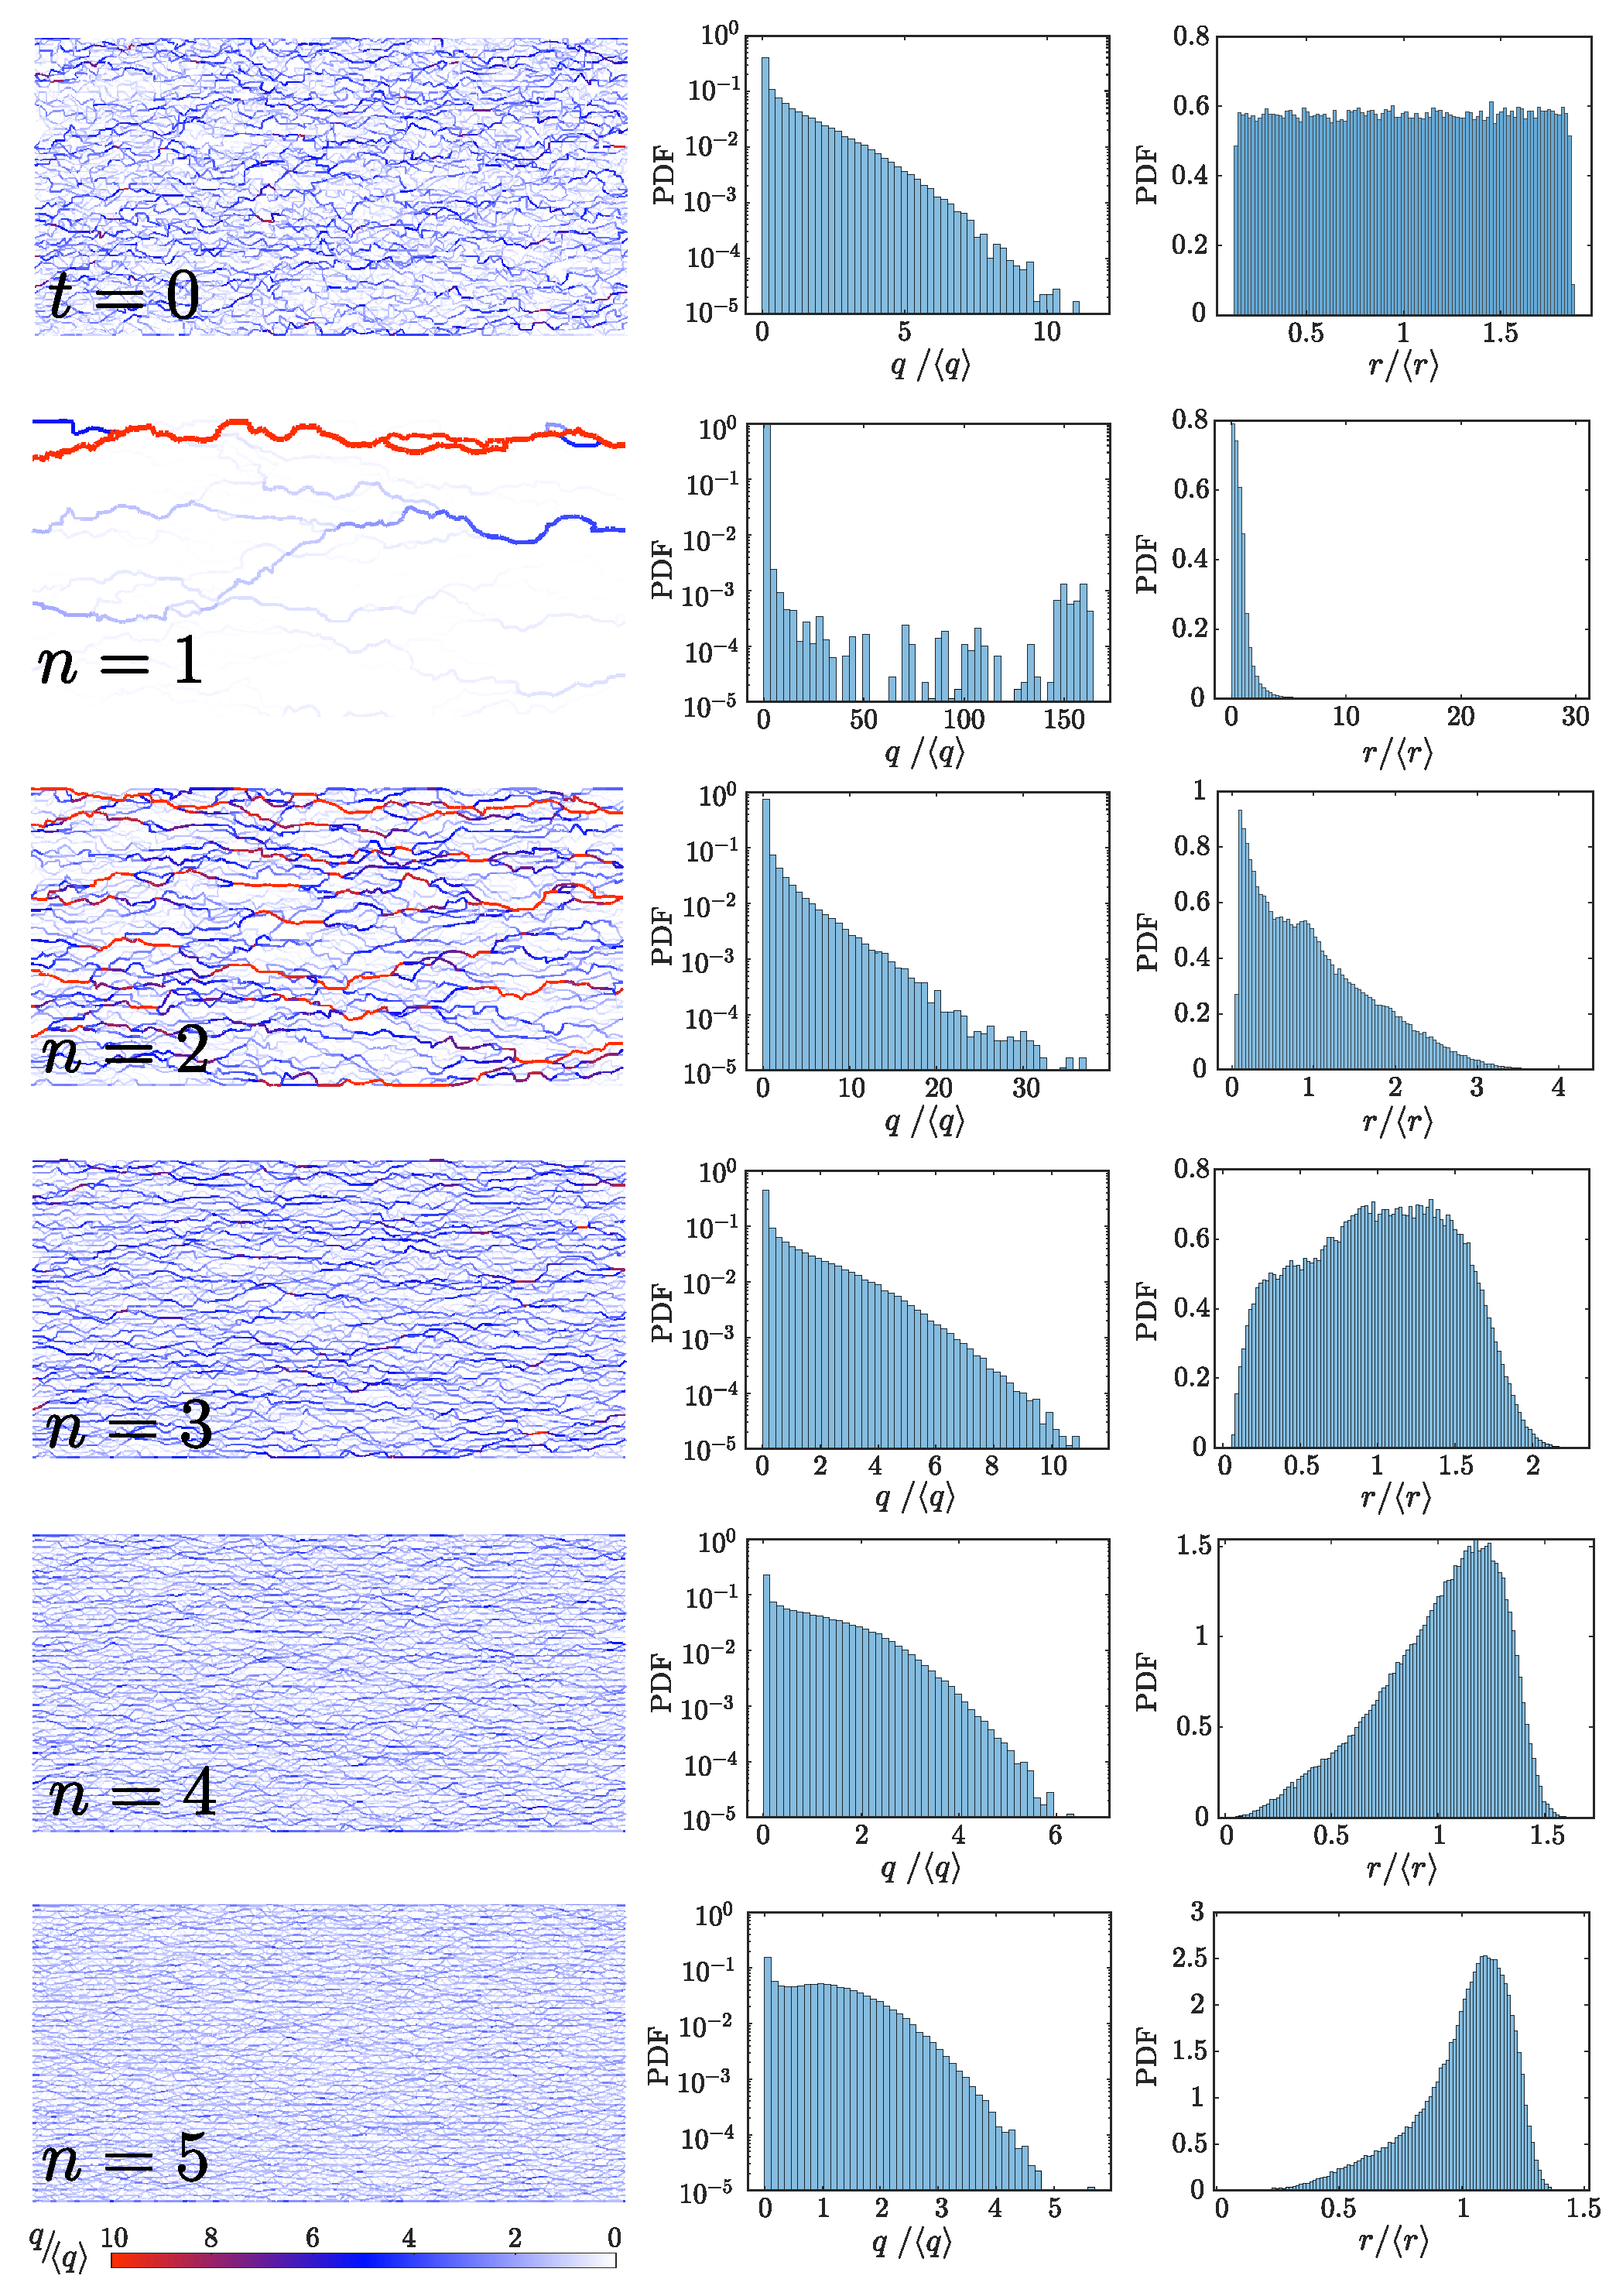
\includegraphics[width = 0.48\textwidth]{Fig2_.pdf}
    \caption{Erosion in a network of pipes. The initial condition is shown with the label $t=0$ in the first row. Each row afterward corresponds to the {simulation result at $t=T$ where  $\langle r_{t=T}\rangle=2r_0$ with $r_0 = \langle r_{t=0}\rangle$}. The erosion law is based on $f(|q|,r) = |q|/r^n$  with different powers of $n$ correspond to different models of erosion. The first, second, and third columns are snapshots of the pore network, the PDF of normalized fluid flux $q/\langle q \rangle$, and  the PDF of normalized radius $r/\langle r\rangle$ at $t=T$, respectively.} \label{fig:fig2}
\end{figure}
%
% 
% \begin{figure*}[htp]
%      % \centering
%       \includegraphics[width = 1.0\textwidth]{FigS2.pdf}
%      \caption{\add{Erosion in a topologically random 3D network of tubes with $N_x=20, N_y=12, N_z=12$ points for Voronoi cell initialization and an initial uniform broad distribution of tube diameters randomly sampled from $\mathcal{U}(1,14)$. Snapshots of the network, PDF of normalized fluid flux $q/\langle q \rangle$, and normalized edge radius distribution $r/\langle r \rangle$ at the initial time $t=0$, and also after $N$ erosion steps for different powers of erosion $n$ are shown. We stop the erosion after $N$ steps such that $\langle r\rangle=2r_0$ where $r_0 = \langle r_{t=0}\rangle$. The erosion law is based on Eq. (1) \del{in the main text} where different powers of $n$ correspond to different models of erosion.}}\label{SIfig:fig2-3d}
%  \end{figure*}
%
% In order to model erosion in porous media, we consider the abrasion in the throats leading to decrease in the tube radii. We model the dynamics as 
%
% \begin{align}
%   \frac{dr_{ij}}{dt} = \alpha  \frac{|q_{ij}|^m}{r_{ij}^n}, \label{eq:erosion-law}
% \end{align}
%
% where $m,n,\alpha$ are constants. Different values of $m$ and $n$ along with a positive $\alpha>0$ correspond to different erosion physics (analogously, $\alpha<0$ corresponds to clogging).
Particularly, the erosion when $m=1$ and  (i) $n=0$ depends on the amount of flux $q_{ij}$ passing through the edge; (ii) $n=2$ depends on the local velocities  \cite{kudrolli2016evolution}; (iii) $n=3$ depends on the shear force at the boundary of the throat~ \cite{bonelli2011micromechanical,parker2000purely,jager2017channelization}. {Additionally, $m=2$ and $n=6$ corresponds to models considered in biological transport networks where the radii changes are {proportional to the square of shear stress at the boundary walls}~\cite{hu2013adaptation,ronellenfitsch2016global}.}  We later address the effect of incorporating the threshold discussed above into our model.  
We consider a randomly initialized network with disordered diameters obtained from a uniform distribution (SM S1). 
The flow inside the pores, PDF of flux in the tubes, and PDF of tube radii are shown in Fig. \ref{fig:fig2}. We assume a constant pressure difference between the left and the right boundaries. In each time step, we increase the local radii of the tubes based on the erosion law $dr_{ij}/dt = \alpha q_{ij}^m/r_{ij}^n$, assuming erosion is linear in the flux ($m=1$). Later we will consider the network behavior for other powers of $m$. 
We continue the simulations until $\langle r \rangle = 2 r_0$. 
The results of the simulations for different values of $n$ are shown in Fig. \ref{fig:fig2}. When $n=1$ or $2$,  the network develops channels. In such cases, the flow is dominated by a few edges carrying most of the flow while the rest of the network carries almost no flow. This is also reflected by a bimodal radii distribution. In contrast, when $n=3$  (corresponding to erosion linear in shear), we find that despite the 
increase in tube radii and absolute flow rates, the normalized flow distribution is hardly affected, maintaining its original exponential form. Increasing $n$ to larger values, $n=4$ or $5$, we find that the flow pattern in the network moves towards homogenization. Here, the tail of the normalized fluid flux distribution retracts and the coefficient of variation reduces. Similarly, the PDF of the tube diameters becomes narrower.  It is to be noted that the different distributions obtained for different powers of $m,n$ represent different statistics that cannot be collapsed.  

We found that similar results uphold in a 3d random tube network  (see SM, Fig.~S2) as well as a 2d topologically ordered (diamond grid) network, illustrating the robustness of the results to the network topology (SM, Fig.~S3). Similarly, we found that the results hold also when using an initial narrow distribution of diameters (SM, Fig.~S4), showing robustness with respect to the strength of the disorder.  We further changed the boundary conditions, using a circular random network with the inlet at the center and outlet at the outer edges and we find that similar results uphold~(SM, Fig.~S5). 

\textit{Phase transition and order parameter}-- {To quantify the transition of the network between the channeling instability and homogenization, we define an order parameter % $\mathcal{O}$ 
%
\begin{align}
\mathcal{O} = \frac{1}{N-1} \left( N - \frac{\left( \sum_{ij} q^2_{ij}\right)^2}{ \sum_{ij} q^4_{ij}}\right),
\end{align}
%
where $N$ is the number of edges.} {The order parameter defined here is inspired by the participation ratio (PR) employed to quantify the localization of an eigenstate in the analysis of Anderson localization~\cite{kramer1993localization}.}  The order parameter $\mathcal{O}=0 $ when the flux through every edge is identical. On the other hand, when fluid flux becomes highly localized with only a few edges with non-zero flux, $\mathcal{O}\to 1$.  We numerically calculated the  order parameter $\mathcal{O}$ for {randomly initialized networks, averaged over 20 different realization}. 
The results are shown in Fig. \ref{fig:fig3}a for different amounts of erosion measured by the increase in the average diameter $\langle r\rangle /r_0$. As shown in 
 Fig. \ref{fig:fig3}c, at $n\approx 3$ the order parameter, remains unchanged; however for $n>3$ the order parameter moves toward zero, where the flow becomes more uniform, and for $n<3$ the order parameter goes toward unity, where channels are developed. This indicates a phase transition at $n=3$ in the long-time behavior of the network.
%


\begin{figure}[!h]
    % \centering
     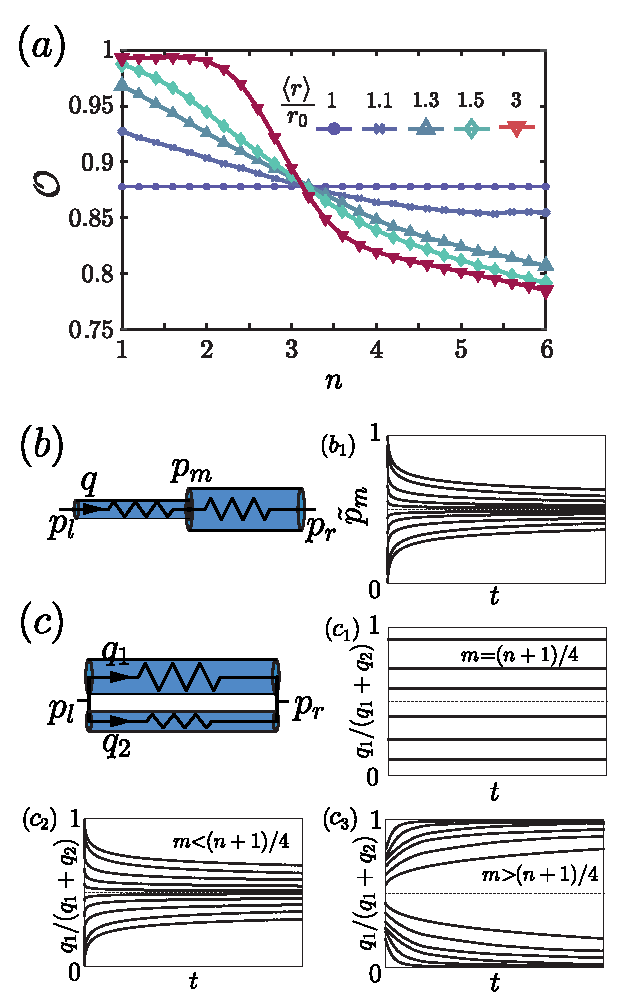
\includegraphics[width = 0.45\textwidth]{Fig3.pdf}
    \caption{ (a) Order parameter $\mathcal{O}$ calculated from simulation results presented in Fig. \ref{fig:fig2} for different powers of $n$ with $m=1$ plotted over time. (b,c) Tubes in series (b) or parallel (c) configuration. 
    The tube radius dynamically change with the erosion law, i.e., $f(q,r) = \alpha |q|^m/r^n$. When the tubes are in series, for any $m,n$, (b$_1$) the normalized pressure at the middle junction between the tubes $\tilde p_m = (p_m - p_l)/(p_r-p_l)$ approaches $1/2$ which results in a homogenized pressure distribution. 
    When the tubes are in parallel, for (c$_1$) $m=(n+1)/4$, the flow ratio between the pipes does not change over time; (c$_2$)  $m<(n+1)/4$ the flow distributes between the tubes equally and  $q_1/(q_1+q_2) \to 1$ which results in the homogenization of the network; (c$_3$) $m>(n+1)/4 $, the entire flow eventually passes through one of the tubes, and channeling occurs. }\label{fig:fig3}
\end{figure}


\textit{Local Dynamics Model}--  To understand the transition in network behavior during erosion, we focus on a simplified model with only two tubes \add{of the same length $L$} in parallel or series with a general erosion dynamics as $dr_{i}/dt = f(q_{i},r_{i}), i=1,2$ (Figs. \ref{fig:fig3}b-c). First, assuming two cylindrical tubes with radii $r_1,r_2$ in series with a given pressure difference of $\delta p = p_r- p_l$, the radius of each tube changes as $dr_i/dt = f(q,r_i),~i=1,2$ (Fig. \ref{fig:fig3}b) where $q=q_1=q_2$. Without loss of generality we assume $r_1>r_2$. Considering the pressure at the junction between tubes $\tilde p_m = (p_m-p_l)/(p_r-p_l)= C_2/(C_1+C_2)$. Time evolution of the middle pressure then follows % 
%
\begin{align}
    \frac{d\tilde{p}_m}{dt} = \gamma (r_1 f(q,r_2)-r_2 f(q,r_1)).
\end{align}
%
where $\gamma = \sqrt{{2\pi}/{\mu L}}{C_1^{\frac{3}{4}} C_2^{\frac{3}{4}}}/{ (C_1+C_2)^2}$. In the above equation, $r_1=r_2$ is a fixed point solution where $d\tilde p_m/dt =0$ and $p_m=1/2$. Since we assumed $r_1>r_2$, we can see that $\tilde p_m <1/2$, and if ${d\tilde{p}_m}/{dt}>0$, then $\tilde p_m \to 1/2$ and the flow homogenizes. Note that if $f(q,r) = \alpha q^m/r^n$, we find that for any $n>0$ the network homogenizes (see Fig. \ref{fig:fig3}b). Contrary to tubes in series, when the tubes are in parallel (Fig. \ref{fig:fig3}c), the net flow $q$ divides between the two tubes in proportion to their conductivity, i.e., $ q_1/q_2 = C_1/C_2$ which results in $q_1/q = \tilde C_1$, where $\tilde C_1 = C_1/(C_1+C_2)$. Note that the dynamics for each pipe in the parallel case can be simplified to $dr_i/dt = g(r_i)$ where $g(r_i) \equiv f(q_i, r_i)$ in which $q_i = \pi r_i^4 \Delta p / 8\mu L$. Given these dynamics, the evolution of the fluid flow ratio becomes $d(q_1/q)/dt = d \tilde C_1/dt= \sqrt{{2\pi}/{\mu L}} \gamma (r_2 g(r_1)-r_1 g(r_2))$. Similarly, it can be seen that  $r_1=r_2$ is a fixed point, where flow is equally distributed between the edges resulting in homogenization. If $d \tilde C_1/dt <0$, then the edge with larger radius has a reduced growth rate while the smaller radius edge has an increasing growth until $r_1=r_2$ is reached. This condition results in homogenization, where both edge's radius increases until the fixed point of $r_1=r_2$ is reached. The condition of $d \tilde C_1/dt<0$ is satisfied when 
%
\begin{align}
    \frac{g(r_1)}{g(r_2)}<\frac{r_1}{r_2}, \quad \forall r_1>r_2>0. \label{eq:condition}
\end{align}
%
\add{In fact, this condition will hold for nonlaminar flow as long as $C \propto r^k (k>0).$ The power law dependence of conductance with respect to radius leads to the scale-free criteria $r_1/r_2$.}
Note that if $d\left(g(r)/r\right)/dr<0$, then Eq.~\eqref{eq:condition} is satisfied, and homogenization would occur. 
The above homogenization condition can further be simplified as $g(r)>g'(r)r$, which can also be obtained directly using a linear stability analysis. Given the homogenization condition $g(r)>g'(r)r$, if the erosion rate is sub-linear locally near the initial radius, the network moves towards homogenization. On the other hand, if the erosion rate is super-linear, we expect the parallel tubes to move away from homogenization and channelization occurs. Applying the power law erosion model with $f(q_{i},r_i)=\alpha q_i^m/r_i^n$, it can be shown that $g(r) \propto  r^{4m-n} $, and therefore $4m-n=1$ results in no change in the flow ratio $q_1/q$ (Fig. \ref{fig:fig3}c$_1$), while $4m-n<1$ results in homogenization condition (Fig.~\ref{fig:fig3}c$_2$), and $4m-n>1$ results in channelization (Fig. \ref{fig:fig3}c$_3$). Since a complex network includes both series and parallel connections, it is plausible that the whole network structure will behave in a similar manner, with an approximate transition in the network's behavior at $ m = (n+1)/4$. This result for $m=1$ reduces to a transition at $n=3$. It is to be noted that while the flow ratio remains constant for parallel edges, the connections in series are evolving toward homogenization and that is why we find a difference between evolved network for $n=3$ and the network at $t=0$. Since series connections are always moving toward homogenization, while parallel connections show a phase transition, we expect the phase transition to be at approximately $n\approx 3$, governed by the parallel connections. This observation  is consistent with the numerical simulation results shown in Figs.~\ref{fig:fig2} and \ref{fig:fig3}a (for $m=1$) as well as for additional values of $m$ (Fig.~\ref{fig:fig4}). Note, however, that the local dynamics model is only approximate and the numerically observed value of the phase transition happens for a value slightly larger than $n=3$ in Fig. \ref{fig:fig3}.
% consistent with the homogenizing effect of the series connections. }
% Although the result is derived under the constant pressure difference assumption, it holds validity for homogenization cases, where the pressure difference is going towards homogenization as well.


% \textit{Simplified Model}-- {To understand the transition in network behavior during erosion for different powers of $n$, we focus on a simplified model with only two tubes in parallel or series (Figs. \ref{fig:fig3}b-c). First, assuming two cylindrical tubes with radii $r_1,r_2$ in series, the flow is the same for the two tubes $ q_1 = q_2 = q$ (Fig. \ref{fig:fig3}b). The radius of each tube then changes as $dr_i/dt = \alpha q^m /r_i^n$ where $i=1,2$. 
% As a result, we find that the conductivity of each tube changes as $dC_i/dt \propto q^m C_i^{(3-n)/4}$, where each tube's conductivity increases. Considering the pressure at the junction between tubes, we find that it moves toward the average value of pressure on both sides (Fig. \ref{fig:fig3}(b$_1$)). Contrary to tubes in series, when the tubes are in parallel (Fig. \ref{fig:fig3}c), the flow divides between the two tubes in proportion to their conductivity, i.e., $q_1/q_2 = C_1/C_2$. Since each tube's radius changes as $dr_i/dt = \alpha q^m_i/r_i^n$, the evolution of the fluid flow ratio becomes 
% % %% 
% \begin{align}
% \frac{d}{dt}\left( \frac{C_1}{C_2}\right) \propto  \frac{C_1}{C^{n/4+1}_2} \left( \left( \frac{C_1}{C_2}\right)^{m-\frac{n+1}{4}} - 1 \right). \label{eq:dyn-paral}
% \end{align}
% %%
% When $m=(n+1)/4$ in Eq. \eqref{eq:dyn-paral}, the right-hand-side vanishes and as a result the flow ratio $C_1/C_2$ remains constant \add{while the radius keeps changing} (Fig.~\ref{fig:fig3}c$_1$). However, when $m \neq (n+1)/4$, we find that $C_1/C_2 = 1$ is an equilibrium point. When $m<(n+1)/4$ this equilibrium solution is stable and the flow moves toward homogenization (Fig. \ref{fig:fig3}c$_2$); however, when $m>(n+1)/4$ this equilibrium solution becomes unstable and the solution moves toward $C_1/C_2 \to 0$ or $\infty$ which means that the entire flow passes through one of the tubes (Fig. \ref{fig:fig3}c$_3$). In summary, when the tubes are in series any erosion law makes flow become more uniform; however, when the tubes are in parallel depending on the powers $m,n$ the flow in the tubes can move toward becoming more uniform ($m<(n+1)/4$), maintain the same ratio ($m=(n+1)/4$), or move toward instability and channel development ($m>(n+1)/4$). {Since a complex network includes both series and parallel connections, it is plausible that the whole network structure will behave in a similar manner, with \add{an approximate} transition in the networks behavior at $ m = (n+1)/4$}. \add{It is to be noted that the series connection are always moving toward homogenization, while only parallel connections showing a phase transition.  As a result, we expect the phase transition to be happening close at approximately $n\approx 3$, where the parallel connections reflect this transition.} This observation  is consistent with the numerical simulation results shown in Figs.~\ref{fig:fig2} and \ref{fig:fig3}a (for $m=1$) as well as for additional values of $m$ (Fig.~\ref{fig:fig4}).} \add{Note that the true phase transition happens for a value slightly smaller than $n=3$ in Fig. \ref{fig:fig3} and the the order parameter for $n=3$ slightly moves toward homogenization. This is due to the fact that the series connections are homogenizing while the parallel connections grow in proportion.} 
% %
% %

\textit{Analysis of generalized model}--  So far we focused on erosion dynamics with $m=1$ in $f(|q_{ij}|,r_{ij})=\alpha |q_{ij}|^m/r_{ij}^n$ since it directly corresponds to erosion laws of interest, i.e. an erosion rate with a linear dependence on fluid-flux, velocity, or shear-rate at the walls. Considering $m=2$, our model aligns with the transport optimization problem in biological networks~\cite{ronellenfitsch2016global,corson2010fluctuations,hu2013adaptation}. 
% Previous works have suggested that in the context of biological transport networks, the network is optimized to minimize its dissipation energy with regards to some constraint (such as constant material or metabolic cost).  Interestingly, the gradient descent method utilized to find the minimal energy configurations maps to Eq. \eqref{eq:erosion-law} with $m=2$, albeit with additional regularizing terms. While under the dynamics we study here erosion will occur indefinitely, in these biological network models a minimal energy configuration exists due to these additional constraints. Nonetheless, the minimal energy configurations manifest a phase transition reminiscent of the one we observe in our model. 
To test the role of the parameter $m$ in our model, we simulated the general form of erosion dynamics with $f(|q_{ij}|,r_{ij}) = \alpha |q_{ij}|^m/r_{ij}^n$.
The simulation results for a randomly initialized network for different powers of $m$ and $n$ are shown in Fig. \ref{fig:fig4}, where each box shows the final snapshot of the network eroded with the corresponding $m$ and $n$. % We further compare the network's simulation result with the simplified model's prediction. for the fate of the network for each pair of $m,n$. 
Additionally, the prediction of the local dynamics model is shown using the bounding box color (red for channelization and green for homogenization) in Fig. \ref{fig:fig4} (cf., Fig.~S8 in SM showing the heat map for the average change in the order parameter). The dashed black line in Fig. \ref{fig:fig4} shows the  the local dynamics model's prediction for the boundary between network's transition to homogeneity or channelization (i.e., $m = (n+1)/4$). 
% Although the simplified model is based on the erosion dynamics of two edges in a parallel or series configuration, it still 
We find that the local dynamics model correctly predicts the fate of the network with the complex topology for different values of $m$ and $n$, and captures the boundary separating channelization/homogenization.  We further consider a model where the onset of erosion happens only after  a certain threshold (see SM \S4 and Figs. S6 and S7) and find that the transition remains unchanged at $m=(n+1)/4$, showing robustness to thresholding effects. Additionally, to further test the generality of the local dynamics model, we used a nonlinear function of shear rate as $dr/dt = h(\tau)$ where $\tau=q/r^3$. We found that the prediction of the local dynamics model matches with the direct simulations (see SM \S7 and Figs. S9 and S10) where it can be used to predict the fate of a network given a general erosion law. 


\begin{figure}[!ht]
    \centering
    \includegraphics[width = 0.45\textwidth]{Fig4.pdf}
    \caption{Evolution of a randomly initialized network for various powers of $m$ and $n$ in $f(|q|,r) = \alpha |q|^m/r^n$. The network is randomly initialized with $50\times 50$ randomly distributed pores. The bounding box color shows the prediction of the local dynamics model for the fate of the network: homogenization (blue) or channelization (red). The dashed black line shows the transition boundary between channelization instability and homogenization obtained using local dynamics model, i.e., $m=(n+1)/4$.}\label{fig:fig4}
\end{figure}
%%%%%%%%%%%%%%%%%%%%%%%%%%%%%%%%%%%%%%%%%%%%%
% 
%%%%%%%%%%%%%%%%%%%%%%%%%%%%%%%%%%%%%%%%%%%%%%%%
In the case of clogging, the initial dynamics can similarly be captured using our model, however, due to the change in the connectivity of the network, our local dynamics model cannot extend to large time behaviors (SM, \S5).
 

%
\textit{Conclusion}-- {We analyzed the dynamics of porous networks during erosion.  We showed that depending on the form of the erosion law (namely, its dependence on flux and tube radius) the network can either move towards homogenization or towards developing a channeling instability.  We elucidated the physical origin of this phase transition and how it is achieved using a simplified model. Our results highlight the importance of local dynamics and feedback mechanisms in the network's path toward its asymptotic global behavior \cite{ronellenfitsch2016global,corson2010fluctuations,katifori2010damage,hu2013adaptation,ocko2015feedback},  and allow us to infer the local dynamics using large scale observations. As a result, our model can be used as a bulk behavior proxy for determining the local dynamics of erosion in a system~\cite{mahadevan2012flow}. Interestingly, our results indicates that an erosion model that is local and linearly dependent on shear rate cannot result in channelization (since $m=1,n=3$ and $m=(n+1)/4$). However, we note that if the dependence on the shear rate is non-linear, it will qualitatively map to our model albeit with renormalized values of $n$ and $m$: e.g., a power-law dependence on shear rate with exponent $s$ would lead to $m =s$, $n = 3 s$, implying channelization when $s>1$. In the future, it would be exciting to test this and other predictions experimentally on model systems, relying on the technological advances in imaging flow profiles in porous materials, as well as extend the study to the geologically relevant case of chemical erosion \cite{edery2014origins,edery2016characterization}, and wormhole formation in geologic formations during CO$_2$ injection \cite{ott2015wormhole,szymczak2009wormhole}. Additionally, the model studied here could become richer by tracking the solute
being eroded through solute concentration using $dr/dt=f(q,r,c)$ where $c$ is the solute concentration, and allow for solute deposition along the porous material~\cite{bizmark2020multiscale,jager2018clogging,jaeger2017mechanism}. 
}



\begin{acknowledgments}
We thank the Kavli Foundation, MRSEC  DMR-2011754, and DMR-1420570 for their support. We thank Yaniv Edery,  Eleni Katifori, and Chris Rycroft
for useful discussions.
\end{acknowledgments}

%%%%%%%%%%%%%%%%%%%%%%%%%%%%%%%%%%%%%%%%%%%%%%%%%
%%%%%%%%%%%%%%%%%%%%%%%%%%%%%%%%%%%%%%%%%%%%%%%%%
%%%%%%%%%%%%%%%%%%%%%%%%%%%%%%%%%%%%%%%%%%%%%%%%%
%%%%%%%%%%%%%%%%%%%%%%%%%%%%%%%%%%%%%%%%%%%%%%%5
%merlin.mbs apsrev4-1.bst 2010-07-25 4.21a (PWD, AO, DPC) hacked
%Control: key (0)
%Control: author (8) initials jnrlst
%Control: editor formatted (1) identically to author
%Control: production of article title (-1) disabled
%Control: page (0) single
%Control: year (1) truncated
%Control: production of eprint (0) enabled
\begin{thebibliography}{58}%
\makeatletter
\providecommand \@ifxundefined [1]{%
 \@ifx{#1\undefined}
}%
\providecommand \@ifnum [1]{%
 \ifnum #1\expandafter \@firstoftwo
 \else \expandafter \@secondoftwo
 \fi
}%
\providecommand \@ifx [1]{%
 \ifx #1\expandafter \@firstoftwo
 \else \expandafter \@secondoftwo
 \fi
}%
\providecommand \natexlab [1]{#1}%
\providecommand \enquote  [1]{``#1''}%
\providecommand \bibnamefont  [1]{#1}%
\providecommand \bibfnamefont [1]{#1}%
\providecommand \citenamefont [1]{#1}%
\providecommand \href@noop [0]{\@secondoftwo}%
\providecommand \href [0]{\begingroup \@sanitize@url \@href}%
\providecommand \@href[1]{\@@startlink{#1}\@@href}%
\providecommand \@@href[1]{\endgroup#1\@@endlink}%
\providecommand \@sanitize@url [0]{\catcode `\\12\catcode `\$12\catcode
  `\&12\catcode `\#12\catcode `\^12\catcode `\_12\catcode `\%12\relax}%
\providecommand \@@startlink[1]{}%
\providecommand \@@endlink[0]{}%
\providecommand \url  [0]{\begingroup\@sanitize@url \@url }%
\providecommand \@url [1]{\endgroup\@href {#1}{\urlprefix }}%
\providecommand \urlprefix  [0]{URL }%
\providecommand \Eprint [0]{\href }%
\providecommand \doibase [0]{http://dx.doi.org/}%
\providecommand \selectlanguage [0]{\@gobble}%
\providecommand \bibinfo  [0]{\@secondoftwo}%
\providecommand \bibfield  [0]{\@secondoftwo}%
\providecommand \translation [1]{[#1]}%
\providecommand \BibitemOpen [0]{}%
\providecommand \bibitemStop [0]{}%
\providecommand \bibitemNoStop [0]{.\EOS\space}%
\providecommand \EOS [0]{\spacefactor3000\relax}%
\providecommand \BibitemShut  [1]{\csname bibitem#1\endcsname}%
\let\auto@bib@innerbib\@empty
%</preamble>
\bibitem [{\citenamefont {Marbach}\ \emph {et~al.}(2016)\citenamefont
  {Marbach}, \citenamefont {Alim}, \citenamefont {Andrew}, \citenamefont
  {Pringle},\ and\ \citenamefont {Brenner}}]{marbach2016pruning}%
  \BibitemOpen
  \bibfield  {author} {\bibinfo {author} {\bibfnamefont {S.}~\bibnamefont
  {Marbach}}, \bibinfo {author} {\bibfnamefont {K.}~\bibnamefont {Alim}},
  \bibinfo {author} {\bibfnamefont {N.}~\bibnamefont {Andrew}}, \bibinfo
  {author} {\bibfnamefont {A.}~\bibnamefont {Pringle}}, \ and\ \bibinfo
  {author} {\bibfnamefont {M.~P.}\ \bibnamefont {Brenner}},\ }\href@noop {}
  {\bibfield  {journal} {\bibinfo  {journal} {Physical Review Letters}\
  }\textbf {\bibinfo {volume} {117}},\ \bibinfo {pages} {178103} (\bibinfo
  {year} {2016})}\BibitemShut {NoStop}%
\bibitem [{\citenamefont {Alim}\ \emph {et~al.}(2013)\citenamefont {Alim},
  \citenamefont {Amselem}, \citenamefont {Peaudecerf}, \citenamefont
  {Brenner},\ and\ \citenamefont {Pringle}}]{alim2013random}%
  \BibitemOpen
  \bibfield  {author} {\bibinfo {author} {\bibfnamefont {K.}~\bibnamefont
  {Alim}}, \bibinfo {author} {\bibfnamefont {G.}~\bibnamefont {Amselem}},
  \bibinfo {author} {\bibfnamefont {F.}~\bibnamefont {Peaudecerf}}, \bibinfo
  {author} {\bibfnamefont {M.~P.}\ \bibnamefont {Brenner}}, \ and\ \bibinfo
  {author} {\bibfnamefont {A.}~\bibnamefont {Pringle}},\ }\href@noop {}
  {\bibfield  {journal} {\bibinfo  {journal} {Proceedings of the National
  Academy of Sciences}\ }\textbf {\bibinfo {volume} {110}},\ \bibinfo {pages}
  {13306} (\bibinfo {year} {2013})}\BibitemShut {NoStop}%
\bibitem [{\citenamefont {Tero}\ \emph {et~al.}(2010)\citenamefont {Tero},
  \citenamefont {Takagi}, \citenamefont {Saigusa}, \citenamefont {Ito},
  \citenamefont {Bebber}, \citenamefont {Fricker}, \citenamefont {Yumiki},
  \citenamefont {Kobayashi},\ and\ \citenamefont {Nakagaki}}]{tero2010rules}%
  \BibitemOpen
  \bibfield  {author} {\bibinfo {author} {\bibfnamefont {A.}~\bibnamefont
  {Tero}}, \bibinfo {author} {\bibfnamefont {S.}~\bibnamefont {Takagi}},
  \bibinfo {author} {\bibfnamefont {T.}~\bibnamefont {Saigusa}}, \bibinfo
  {author} {\bibfnamefont {K.}~\bibnamefont {Ito}}, \bibinfo {author}
  {\bibfnamefont {D.~P.}\ \bibnamefont {Bebber}}, \bibinfo {author}
  {\bibfnamefont {M.~D.}\ \bibnamefont {Fricker}}, \bibinfo {author}
  {\bibfnamefont {K.}~\bibnamefont {Yumiki}}, \bibinfo {author} {\bibfnamefont
  {R.}~\bibnamefont {Kobayashi}}, \ and\ \bibinfo {author} {\bibfnamefont
  {T.}~\bibnamefont {Nakagaki}},\ }\href@noop {} {\bibfield  {journal}
  {\bibinfo  {journal} {Science}\ }\textbf {\bibinfo {volume} {327}},\ \bibinfo
  {pages} {439} (\bibinfo {year} {2010})}\BibitemShut {NoStop}%
\bibitem [{\citenamefont {Heaton}\ \emph {et~al.}(2010)\citenamefont {Heaton},
  \citenamefont {L{\'o}pez}, \citenamefont {Maini}, \citenamefont {Fricker},\
  and\ \citenamefont {Jones}}]{heaton2010growth}%
  \BibitemOpen
  \bibfield  {author} {\bibinfo {author} {\bibfnamefont {L.~L.}\ \bibnamefont
  {Heaton}}, \bibinfo {author} {\bibfnamefont {E.}~\bibnamefont {L{\'o}pez}},
  \bibinfo {author} {\bibfnamefont {P.~K.}\ \bibnamefont {Maini}}, \bibinfo
  {author} {\bibfnamefont {M.~D.}\ \bibnamefont {Fricker}}, \ and\ \bibinfo
  {author} {\bibfnamefont {N.~S.}\ \bibnamefont {Jones}},\ }\href@noop {}
  {\bibfield  {journal} {\bibinfo  {journal} {Proceedings of the Royal Society
  B: Biological Sciences}\ }\textbf {\bibinfo {volume} {277}},\ \bibinfo
  {pages} {3265} (\bibinfo {year} {2010})}\BibitemShut {NoStop}%
\bibitem [{\citenamefont {Schlesinger}(1999)}]{schlesinger1999carbon}%
  \BibitemOpen
  \bibfield  {author} {\bibinfo {author} {\bibfnamefont {W.~H.}\ \bibnamefont
  {Schlesinger}},\ }\href@noop {} {\bibfield  {journal} {\bibinfo  {journal}
  {Science}\ }\textbf {\bibinfo {volume} {284}},\ \bibinfo {pages} {2095}
  (\bibinfo {year} {1999})}\BibitemShut {NoStop}%
\bibitem [{\citenamefont {Winkler}\ and\ \citenamefont
  {Nur}(1979)}]{winkler1979pore}%
  \BibitemOpen
  \bibfield  {author} {\bibinfo {author} {\bibfnamefont {K.}~\bibnamefont
  {Winkler}}\ and\ \bibinfo {author} {\bibfnamefont {A.}~\bibnamefont {Nur}},\
  }\href@noop {} {\bibfield  {journal} {\bibinfo  {journal} {Geophysical
  Research Letters}\ }\textbf {\bibinfo {volume} {6}},\ \bibinfo {pages} {1}
  (\bibinfo {year} {1979})}\BibitemShut {NoStop}%
\bibitem [{\citenamefont {Batzle}\ and\ \citenamefont
  {Wang}(1992)}]{batzle1992seismic}%
  \BibitemOpen
  \bibfield  {author} {\bibinfo {author} {\bibfnamefont {M.}~\bibnamefont
  {Batzle}}\ and\ \bibinfo {author} {\bibfnamefont {Z.}~\bibnamefont {Wang}},\
  }\href@noop {} {\bibfield  {journal} {\bibinfo  {journal} {Geophysics}\
  }\textbf {\bibinfo {volume} {57}},\ \bibinfo {pages} {1396} (\bibinfo {year}
  {1992})}\BibitemShut {NoStop}%
\bibitem [{\citenamefont {Cohen}\ and\ \citenamefont
  {Rothman}(2015)}]{cohen2015mechanisms}%
  \BibitemOpen
  \bibfield  {author} {\bibinfo {author} {\bibfnamefont {Y.}~\bibnamefont
  {Cohen}}\ and\ \bibinfo {author} {\bibfnamefont {D.~H.}\ \bibnamefont
  {Rothman}},\ }\href@noop {} {\bibfield  {journal} {\bibinfo  {journal}
  {Proceedings of the Royal Society A: Mathematical, Physical and Engineering
  Sciences}\ }\textbf {\bibinfo {volume} {471}},\ \bibinfo {pages} {20140853}
  (\bibinfo {year} {2015})}\BibitemShut {NoStop}%
\bibitem [{\citenamefont {Duduta}\ \emph {et~al.}(2011)\citenamefont {Duduta},
  \citenamefont {Ho}, \citenamefont {Wood}, \citenamefont {Limthongkul},
  \citenamefont {Brunini}, \citenamefont {Carter},\ and\ \citenamefont
  {Chiang}}]{duduta2011semi}%
  \BibitemOpen
  \bibfield  {author} {\bibinfo {author} {\bibfnamefont {M.}~\bibnamefont
  {Duduta}}, \bibinfo {author} {\bibfnamefont {B.}~\bibnamefont {Ho}}, \bibinfo
  {author} {\bibfnamefont {V.~C.}\ \bibnamefont {Wood}}, \bibinfo {author}
  {\bibfnamefont {P.}~\bibnamefont {Limthongkul}}, \bibinfo {author}
  {\bibfnamefont {V.~E.}\ \bibnamefont {Brunini}}, \bibinfo {author}
  {\bibfnamefont {W.~C.}\ \bibnamefont {Carter}}, \ and\ \bibinfo {author}
  {\bibfnamefont {Y.-M.}\ \bibnamefont {Chiang}},\ }\href@noop {} {\bibfield
  {journal} {\bibinfo  {journal} {Advanced Energy Materials}\ }\textbf
  {\bibinfo {volume} {1}},\ \bibinfo {pages} {511} (\bibinfo {year}
  {2011})}\BibitemShut {NoStop}%
\bibitem [{\citenamefont {Sun}\ \emph {et~al.}(2019)\citenamefont {Sun},
  \citenamefont {Zhu}, \citenamefont {Baumann}, \citenamefont {Peng},
  \citenamefont {Xu}, \citenamefont {Shakir}, \citenamefont {Huang},\ and\
  \citenamefont {Duan}}]{sun2019hierarchical}%
  \BibitemOpen
  \bibfield  {author} {\bibinfo {author} {\bibfnamefont {H.}~\bibnamefont
  {Sun}}, \bibinfo {author} {\bibfnamefont {J.}~\bibnamefont {Zhu}}, \bibinfo
  {author} {\bibfnamefont {D.}~\bibnamefont {Baumann}}, \bibinfo {author}
  {\bibfnamefont {L.}~\bibnamefont {Peng}}, \bibinfo {author} {\bibfnamefont
  {Y.}~\bibnamefont {Xu}}, \bibinfo {author} {\bibfnamefont {I.}~\bibnamefont
  {Shakir}}, \bibinfo {author} {\bibfnamefont {Y.}~\bibnamefont {Huang}}, \
  and\ \bibinfo {author} {\bibfnamefont {X.}~\bibnamefont {Duan}},\ }\href@noop
  {} {\bibfield  {journal} {\bibinfo  {journal} {Nature Reviews Materials}\
  }\textbf {\bibinfo {volume} {4}},\ \bibinfo {pages} {45} (\bibinfo {year}
  {2019})}\BibitemShut {NoStop}%
\bibitem [{\citenamefont {Smith}\ and\ \citenamefont
  {Bazant}(2017)}]{smith2017multiphase}%
  \BibitemOpen
  \bibfield  {author} {\bibinfo {author} {\bibfnamefont {R.~B.}\ \bibnamefont
  {Smith}}\ and\ \bibinfo {author} {\bibfnamefont {M.~Z.}\ \bibnamefont
  {Bazant}},\ }\href@noop {} {\bibfield  {journal} {\bibinfo  {journal}
  {Journal of The Electrochemical Society}\ }\textbf {\bibinfo {volume}
  {164}},\ \bibinfo {pages} {E3291} (\bibinfo {year} {2017})}\BibitemShut
  {NoStop}%
\bibitem [{\citenamefont {Ferguson}\ and\ \citenamefont
  {Bazant}(2012)}]{ferguson2012nonequilibrium}%
  \BibitemOpen
  \bibfield  {author} {\bibinfo {author} {\bibfnamefont {T.~R.}\ \bibnamefont
  {Ferguson}}\ and\ \bibinfo {author} {\bibfnamefont {M.~Z.}\ \bibnamefont
  {Bazant}},\ }\href@noop {} {\bibfield  {journal} {\bibinfo  {journal}
  {Journal of The Electrochemical Society}\ }\textbf {\bibinfo {volume}
  {159}},\ \bibinfo {pages} {A1967} (\bibinfo {year} {2012})}\BibitemShut
  {NoStop}%
\bibitem [{\citenamefont {Rad}\ \emph {et~al.}(2013)\citenamefont {Rad},
  \citenamefont {Shokri},\ and\ \citenamefont {Sahimi}}]{rad2013pore}%
  \BibitemOpen
  \bibfield  {author} {\bibinfo {author} {\bibfnamefont {M.~N.}\ \bibnamefont
  {Rad}}, \bibinfo {author} {\bibfnamefont {N.}~\bibnamefont {Shokri}}, \ and\
  \bibinfo {author} {\bibfnamefont {M.}~\bibnamefont {Sahimi}},\ }\href@noop {}
  {\bibfield  {journal} {\bibinfo  {journal} {Physical Review E}\ }\textbf
  {\bibinfo {volume} {88}},\ \bibinfo {pages} {032404} (\bibinfo {year}
  {2013})}\BibitemShut {NoStop}%
\bibitem [{\citenamefont {Herzig}\ \emph {et~al.}(1970)\citenamefont {Herzig},
  \citenamefont {Leclerc},\ and\ \citenamefont {Goff}}]{herzig1970flow}%
  \BibitemOpen
  \bibfield  {author} {\bibinfo {author} {\bibfnamefont {J.}~\bibnamefont
  {Herzig}}, \bibinfo {author} {\bibfnamefont {D.}~\bibnamefont {Leclerc}}, \
  and\ \bibinfo {author} {\bibfnamefont {P.~L.}\ \bibnamefont {Goff}},\
  }\href@noop {} {\bibfield  {journal} {\bibinfo  {journal} {Industrial \&
  Engineering Chemistry}\ }\textbf {\bibinfo {volume} {62}},\ \bibinfo {pages}
  {8} (\bibinfo {year} {1970})}\BibitemShut {NoStop}%
\bibitem [{\citenamefont {Tien}\ and\ \citenamefont
  {Payatakes}(1979)}]{tien1979advances}%
  \BibitemOpen
  \bibfield  {author} {\bibinfo {author} {\bibfnamefont {C.}~\bibnamefont
  {Tien}}\ and\ \bibinfo {author} {\bibfnamefont {A.~C.}\ \bibnamefont
  {Payatakes}},\ }\href@noop {} {\bibfield  {journal} {\bibinfo  {journal}
  {AIChE Journal}\ }\textbf {\bibinfo {volume} {25}},\ \bibinfo {pages} {737}
  (\bibinfo {year} {1979})}\BibitemShut {NoStop}%
\bibitem [{\citenamefont {Jaisi}\ \emph {et~al.}(2008)\citenamefont {Jaisi},
  \citenamefont {Saleh}, \citenamefont {Blake},\ and\ \citenamefont
  {Elimelech}}]{jaisi2008transport}%
  \BibitemOpen
  \bibfield  {author} {\bibinfo {author} {\bibfnamefont {D.~P.}\ \bibnamefont
  {Jaisi}}, \bibinfo {author} {\bibfnamefont {N.~B.}\ \bibnamefont {Saleh}},
  \bibinfo {author} {\bibfnamefont {R.~E.}\ \bibnamefont {Blake}}, \ and\
  \bibinfo {author} {\bibfnamefont {M.}~\bibnamefont {Elimelech}},\ }\href@noop
  {} {\bibfield  {journal} {\bibinfo  {journal} {Environmental Science \&
  Technology}\ }\textbf {\bibinfo {volume} {42}},\ \bibinfo {pages} {8317}
  (\bibinfo {year} {2008})}\BibitemShut {NoStop}%
\bibitem [{\citenamefont {Carrel}\ \emph {et~al.}(2018)\citenamefont {Carrel},
  \citenamefont {Morales}, \citenamefont {Beltran}, \citenamefont {Derlon},
  \citenamefont {Kaufmann}, \citenamefont {Morgenroth},\ and\ \citenamefont
  {Holzner}}]{carrel2018biofilms}%
  \BibitemOpen
  \bibfield  {author} {\bibinfo {author} {\bibfnamefont {M.}~\bibnamefont
  {Carrel}}, \bibinfo {author} {\bibfnamefont {V.~L.}\ \bibnamefont {Morales}},
  \bibinfo {author} {\bibfnamefont {M.~A.}\ \bibnamefont {Beltran}}, \bibinfo
  {author} {\bibfnamefont {N.}~\bibnamefont {Derlon}}, \bibinfo {author}
  {\bibfnamefont {R.}~\bibnamefont {Kaufmann}}, \bibinfo {author}
  {\bibfnamefont {E.}~\bibnamefont {Morgenroth}}, \ and\ \bibinfo {author}
  {\bibfnamefont {M.}~\bibnamefont {Holzner}},\ }\href@noop {} {\bibfield
  {journal} {\bibinfo  {journal} {Water Research}\ }\textbf {\bibinfo {volume}
  {134}},\ \bibinfo {pages} {280} (\bibinfo {year} {2018})}\BibitemShut
  {NoStop}%
\bibitem [{\citenamefont {Seymour}\ \emph {et~al.}(2004)\citenamefont
  {Seymour}, \citenamefont {Gage}, \citenamefont {Codd},\ and\ \citenamefont
  {Gerlach}}]{seymour2004anomalous}%
  \BibitemOpen
  \bibfield  {author} {\bibinfo {author} {\bibfnamefont {J.~D.}\ \bibnamefont
  {Seymour}}, \bibinfo {author} {\bibfnamefont {J.~P.}\ \bibnamefont {Gage}},
  \bibinfo {author} {\bibfnamefont {S.~L.}\ \bibnamefont {Codd}}, \ and\
  \bibinfo {author} {\bibfnamefont {R.}~\bibnamefont {Gerlach}},\ }\href@noop
  {} {\bibfield  {journal} {\bibinfo  {journal} {Physical Review Letters}\
  }\textbf {\bibinfo {volume} {93}},\ \bibinfo {pages} {198103} (\bibinfo
  {year} {2004})}\BibitemShut {NoStop}%
\bibitem [{\citenamefont {Lake}\ \emph {et~al.}(2014)\citenamefont {Lake},
  \citenamefont {Johns}, \citenamefont {Rossen}, \citenamefont {Pope} \emph
  {et~al.}}]{lake2014fundamentals}%
  \BibitemOpen
  \bibfield  {author} {\bibinfo {author} {\bibfnamefont {L.~W.}\ \bibnamefont
  {Lake}}, \bibinfo {author} {\bibfnamefont {R.}~\bibnamefont {Johns}},
  \bibinfo {author} {\bibfnamefont {B.}~\bibnamefont {Rossen}}, \bibinfo
  {author} {\bibfnamefont {G.~A.}\ \bibnamefont {Pope}},  \emph {et~al.},\
  }\bibfield  {booktitle} {\emph {\bibinfo {booktitle} {Fundamentals of
  Enhanced Oil Recovery}},\ }\href@noop {} {\  (\bibinfo {year}
  {2014})}\BibitemShut {NoStop}%
\bibitem [{\citenamefont {Parsa}\ \emph {et~al.}(2020)\citenamefont {Parsa},
  \citenamefont {Santanach-Carreras}, \citenamefont {Xiao},\ and\ \citenamefont
  {Weitz}}]{parsa2020origin}%
  \BibitemOpen
  \bibfield  {author} {\bibinfo {author} {\bibfnamefont {S.}~\bibnamefont
  {Parsa}}, \bibinfo {author} {\bibfnamefont {E.}~\bibnamefont
  {Santanach-Carreras}}, \bibinfo {author} {\bibfnamefont {L.}~\bibnamefont
  {Xiao}}, \ and\ \bibinfo {author} {\bibfnamefont {D.~A.}\ \bibnamefont
  {Weitz}},\ }\href@noop {} {\bibfield  {journal} {\bibinfo  {journal}
  {Physical Review Fluids}\ }\textbf {\bibinfo {volume} {5}},\ \bibinfo {pages}
  {022001} (\bibinfo {year} {2020})}\BibitemShut {NoStop}%
\bibitem [{\citenamefont {Schorghofer}\ \emph {et~al.}(2004)\citenamefont
  {Schorghofer}, \citenamefont {Jensen}, \citenamefont {Kudrolli},\ and\
  \citenamefont {Rothman}}]{schorghofer2004spontaneous}%
  \BibitemOpen
  \bibfield  {author} {\bibinfo {author} {\bibfnamefont {N.}~\bibnamefont
  {Schorghofer}}, \bibinfo {author} {\bibfnamefont {B.}~\bibnamefont {Jensen}},
  \bibinfo {author} {\bibfnamefont {A.}~\bibnamefont {Kudrolli}}, \ and\
  \bibinfo {author} {\bibfnamefont {D.~H.}\ \bibnamefont {Rothman}},\
  }\href@noop {} {\bibfield  {journal} {\bibinfo  {journal} {Journal of Fluid
  Mechanics}\ }\textbf {\bibinfo {volume} {503}},\ \bibinfo {pages} {357}
  (\bibinfo {year} {2004})}\BibitemShut {NoStop}%
\bibitem [{\citenamefont {Mahadevan}\ \emph {et~al.}(2012)\citenamefont
  {Mahadevan}, \citenamefont {Orpe}, \citenamefont {Kudrolli},\ and\
  \citenamefont {Mahadevan}}]{mahadevan2012flow}%
  \BibitemOpen
  \bibfield  {author} {\bibinfo {author} {\bibfnamefont {A.}~\bibnamefont
  {Mahadevan}}, \bibinfo {author} {\bibfnamefont {A.}~\bibnamefont {Orpe}},
  \bibinfo {author} {\bibfnamefont {A.}~\bibnamefont {Kudrolli}}, \ and\
  \bibinfo {author} {\bibfnamefont {L.}~\bibnamefont {Mahadevan}},\ }\href@noop
  {} {\bibfield  {journal} {\bibinfo  {journal} {Europhysics Letters}\ }\textbf
  {\bibinfo {volume} {98}},\ \bibinfo {pages} {58003} (\bibinfo {year}
  {2012})}\BibitemShut {NoStop}%
\bibitem [{\citenamefont {Akanji}\ and\ \citenamefont
  {Matthai}(2010)}]{akanji2010finite}%
  \BibitemOpen
  \bibfield  {author} {\bibinfo {author} {\bibfnamefont {L.~T.}\ \bibnamefont
  {Akanji}}\ and\ \bibinfo {author} {\bibfnamefont {S.~K.}\ \bibnamefont
  {Matthai}},\ }\href@noop {} {\bibfield  {journal} {\bibinfo  {journal}
  {Transport in Porous Media}\ }\textbf {\bibinfo {volume} {81}},\ \bibinfo
  {pages} {241} (\bibinfo {year} {2010})}\BibitemShut {NoStop}%
\bibitem [{\citenamefont {Fatt}\ \emph {et~al.}(1956)\citenamefont {Fatt} \emph
  {et~al.}}]{fatt1956network}%
  \BibitemOpen
  \bibfield  {author} {\bibinfo {author} {\bibfnamefont {I.}~\bibnamefont
  {Fatt}} \emph {et~al.},\ }\href@noop {} {\bibfield  {journal} {\bibinfo
  {journal} {Transactions of the AIME}\ }\textbf {\bibinfo {volume} {207}},\
  \bibinfo {pages} {144} (\bibinfo {year} {1956})}\BibitemShut {NoStop}%
\bibitem [{\citenamefont {Blunt}\ \emph {et~al.}(2013)\citenamefont {Blunt},
  \citenamefont {Bijeljic}, \citenamefont {Dong}, \citenamefont {Gharbi},
  \citenamefont {Iglauer}, \citenamefont {Mostaghimi}, \citenamefont
  {Paluszny},\ and\ \citenamefont {Pentland}}]{blunt2013pore}%
  \BibitemOpen
  \bibfield  {author} {\bibinfo {author} {\bibfnamefont {M.~J.}\ \bibnamefont
  {Blunt}}, \bibinfo {author} {\bibfnamefont {B.}~\bibnamefont {Bijeljic}},
  \bibinfo {author} {\bibfnamefont {H.}~\bibnamefont {Dong}}, \bibinfo {author}
  {\bibfnamefont {O.}~\bibnamefont {Gharbi}}, \bibinfo {author} {\bibfnamefont
  {S.}~\bibnamefont {Iglauer}}, \bibinfo {author} {\bibfnamefont
  {P.}~\bibnamefont {Mostaghimi}}, \bibinfo {author} {\bibfnamefont
  {A.}~\bibnamefont {Paluszny}}, \ and\ \bibinfo {author} {\bibfnamefont
  {C.}~\bibnamefont {Pentland}},\ }\href@noop {} {\bibfield  {journal}
  {\bibinfo  {journal} {Advances in Water Resources}\ }\textbf {\bibinfo
  {volume} {51}},\ \bibinfo {pages} {197} (\bibinfo {year} {2013})}\BibitemShut
  {NoStop}%
\bibitem [{\citenamefont {Stoop}\ \emph {et~al.}(2019)\citenamefont {Stoop},
  \citenamefont {Waisbord}, \citenamefont {Kantsler}, \citenamefont {Heinonen},
  \citenamefont {Guasto},\ and\ \citenamefont {Dunkel}}]{stoop2019disorder}%
  \BibitemOpen
  \bibfield  {author} {\bibinfo {author} {\bibfnamefont {N.}~\bibnamefont
  {Stoop}}, \bibinfo {author} {\bibfnamefont {N.}~\bibnamefont {Waisbord}},
  \bibinfo {author} {\bibfnamefont {V.}~\bibnamefont {Kantsler}}, \bibinfo
  {author} {\bibfnamefont {V.}~\bibnamefont {Heinonen}}, \bibinfo {author}
  {\bibfnamefont {J.~S.}\ \bibnamefont {Guasto}}, \ and\ \bibinfo {author}
  {\bibfnamefont {J.}~\bibnamefont {Dunkel}},\ }\href@noop {} {\bibfield
  {journal} {\bibinfo  {journal} {Journal of Non-Newtonian Fluid Mechanics}\
  }\textbf {\bibinfo {volume} {268}},\ \bibinfo {pages} {66} (\bibinfo {year}
  {2019})}\BibitemShut {NoStop}%
\bibitem [{\citenamefont {Bryant}\ \emph {et~al.}(1993)\citenamefont {Bryant},
  \citenamefont {King},\ and\ \citenamefont {Mellor}}]{bryant1993network}%
  \BibitemOpen
  \bibfield  {author} {\bibinfo {author} {\bibfnamefont {S.~L.}\ \bibnamefont
  {Bryant}}, \bibinfo {author} {\bibfnamefont {P.~R.}\ \bibnamefont {King}}, \
  and\ \bibinfo {author} {\bibfnamefont {D.~W.}\ \bibnamefont {Mellor}},\
  }\href@noop {} {\bibfield  {journal} {\bibinfo  {journal} {Transport in
  Porous Media}\ }\textbf {\bibinfo {volume} {11}},\ \bibinfo {pages} {53}
  (\bibinfo {year} {1993})}\BibitemShut {NoStop}%
\bibitem [{\citenamefont {Dong}\ and\ \citenamefont
  {Blunt}(2009)}]{dong2009pore}%
  \BibitemOpen
  \bibfield  {author} {\bibinfo {author} {\bibfnamefont {H.}~\bibnamefont
  {Dong}}\ and\ \bibinfo {author} {\bibfnamefont {M.~J.}\ \bibnamefont
  {Blunt}},\ }\href@noop {} {\bibfield  {journal} {\bibinfo  {journal}
  {Physical Review E}\ }\textbf {\bibinfo {volume} {80}},\ \bibinfo {pages}
  {036307} (\bibinfo {year} {2009})}\BibitemShut {NoStop}%
\bibitem [{\citenamefont {Blunt}\ and\ \citenamefont
  {Scher}(1995)}]{blunt1995pore}%
  \BibitemOpen
  \bibfield  {author} {\bibinfo {author} {\bibfnamefont {M.~J.}\ \bibnamefont
  {Blunt}}\ and\ \bibinfo {author} {\bibfnamefont {H.}~\bibnamefont {Scher}},\
  }\href@noop {} {\bibfield  {journal} {\bibinfo  {journal} {Physical Review
  E}\ }\textbf {\bibinfo {volume} {52}},\ \bibinfo {pages} {6387} (\bibinfo
  {year} {1995})}\BibitemShut {NoStop}%
\bibitem [{\citenamefont {Alim}\ \emph {et~al.}(2017)\citenamefont {Alim},
  \citenamefont {Parsa}, \citenamefont {Weitz},\ and\ \citenamefont
  {Brenner}}]{alim2017local}%
  \BibitemOpen
  \bibfield  {author} {\bibinfo {author} {\bibfnamefont {K.}~\bibnamefont
  {Alim}}, \bibinfo {author} {\bibfnamefont {S.}~\bibnamefont {Parsa}},
  \bibinfo {author} {\bibfnamefont {D.~A.}\ \bibnamefont {Weitz}}, \ and\
  \bibinfo {author} {\bibfnamefont {M.~P.}\ \bibnamefont {Brenner}},\
  }\href@noop {} {\bibfield  {journal} {\bibinfo  {journal} {Physical Review
  Letters}\ }\textbf {\bibinfo {volume} {119}},\ \bibinfo {pages} {144501}
  (\bibinfo {year} {2017})}\BibitemShut {NoStop}%
\bibitem [{\citenamefont {Parsa}\ \emph {et~al.}(2021)\citenamefont {Parsa},
  \citenamefont {Zareei}, \citenamefont {Santanach-Carreras}, \citenamefont
  {Morris}, \citenamefont {Amir}, \citenamefont {Xiao},\ and\ \citenamefont
  {Weitz}}]{shima2021}%
  \BibitemOpen
  \bibfield  {author} {\bibinfo {author} {\bibfnamefont {S.}~\bibnamefont
  {Parsa}}, \bibinfo {author} {\bibfnamefont {A.}~\bibnamefont {Zareei}},
  \bibinfo {author} {\bibfnamefont {E.}~\bibnamefont {Santanach-Carreras}},
  \bibinfo {author} {\bibfnamefont {E.~J.}\ \bibnamefont {Morris}}, \bibinfo
  {author} {\bibfnamefont {A.}~\bibnamefont {Amir}}, \bibinfo {author}
  {\bibfnamefont {L.}~\bibnamefont {Xiao}}, \ and\ \bibinfo {author}
  {\bibfnamefont {D.~A.}\ \bibnamefont {Weitz}},\ }\href@noop {} {\bibfield
  {journal} {\bibinfo  {journal} {Physical Review Fluids}\ }\textbf {\bibinfo
  {volume} {6}},\ \bibinfo {pages} {L082302} (\bibinfo {year}
  {2021})}\BibitemShut {NoStop}%
\bibitem [{\citenamefont {Fraggedakis}\ \emph {et~al.}(2021)\citenamefont
  {Fraggedakis}, \citenamefont {Chaparian},\ and\ \citenamefont
  {Tammisola}}]{fraggedakis_chaparian_tammisola_2021}%
  \BibitemOpen
  \bibfield  {author} {\bibinfo {author} {\bibfnamefont {D.}~\bibnamefont
  {Fraggedakis}}, \bibinfo {author} {\bibfnamefont {E.}~\bibnamefont
  {Chaparian}}, \ and\ \bibinfo {author} {\bibfnamefont {O.}~\bibnamefont
  {Tammisola}},\ }\href@noop {} {\bibfield  {journal} {\bibinfo  {journal}
  {Journal of Fluid Mechanics}\ }\textbf {\bibinfo {volume} {911}},\ \bibinfo
  {pages} {A58} (\bibinfo {year} {2021})}\BibitemShut {NoStop}%
\bibitem [{\citenamefont {Datta}\ \emph {et~al.}(2013)\citenamefont {Datta},
  \citenamefont {Chiang}, \citenamefont {Ramakrishnan},\ and\ \citenamefont
  {Weitz}}]{datta2013spatial}%
  \BibitemOpen
  \bibfield  {author} {\bibinfo {author} {\bibfnamefont {S.~S.}\ \bibnamefont
  {Datta}}, \bibinfo {author} {\bibfnamefont {H.}~\bibnamefont {Chiang}},
  \bibinfo {author} {\bibfnamefont {T.}~\bibnamefont {Ramakrishnan}}, \ and\
  \bibinfo {author} {\bibfnamefont {D.~A.}\ \bibnamefont {Weitz}},\ }\href@noop
  {} {\bibfield  {journal} {\bibinfo  {journal} {Physical Review Letters}\
  }\textbf {\bibinfo {volume} {111}},\ \bibinfo {pages} {064501} (\bibinfo
  {year} {2013})}\BibitemShut {NoStop}%
\bibitem [{\citenamefont {J{\"a}ger}\ \emph {et~al.}(2017)\citenamefont
  {J{\"a}ger}, \citenamefont {Mendoza},\ and\ \citenamefont
  {Herrmann}}]{jager2017channelization}%
  \BibitemOpen
  \bibfield  {author} {\bibinfo {author} {\bibfnamefont {R.}~\bibnamefont
  {J{\"a}ger}}, \bibinfo {author} {\bibfnamefont {M.}~\bibnamefont {Mendoza}},
  \ and\ \bibinfo {author} {\bibfnamefont {H.~J.}\ \bibnamefont {Herrmann}},\
  }\href@noop {} {\bibfield  {journal} {\bibinfo  {journal} {Physical Review
  E}\ }\textbf {\bibinfo {volume} {95}},\ \bibinfo {pages} {013110} (\bibinfo
  {year} {2017})}\BibitemShut {NoStop}%
\bibitem [{\citenamefont {Ristroph}\ \emph {et~al.}(2012)\citenamefont
  {Ristroph}, \citenamefont {Moore}, \citenamefont {Childress}, \citenamefont
  {Shelley},\ and\ \citenamefont {Zhang}}]{ristroph2012sculpting}%
  \BibitemOpen
  \bibfield  {author} {\bibinfo {author} {\bibfnamefont {L.}~\bibnamefont
  {Ristroph}}, \bibinfo {author} {\bibfnamefont {M.~N.}\ \bibnamefont {Moore}},
  \bibinfo {author} {\bibfnamefont {S.}~\bibnamefont {Childress}}, \bibinfo
  {author} {\bibfnamefont {M.~J.}\ \bibnamefont {Shelley}}, \ and\ \bibinfo
  {author} {\bibfnamefont {J.}~\bibnamefont {Zhang}},\ }\href@noop {}
  {\bibfield  {journal} {\bibinfo  {journal} {Proceedings of the National
  Academy of Sciences}\ }\textbf {\bibinfo {volume} {109}},\ \bibinfo {pages}
  {19606} (\bibinfo {year} {2012})}\BibitemShut {NoStop}%
\bibitem [{\citenamefont {Wan}\ and\ \citenamefont
  {Fell}(2004)}]{wan2004investigation}%
  \BibitemOpen
  \bibfield  {author} {\bibinfo {author} {\bibfnamefont {C.~F.}\ \bibnamefont
  {Wan}}\ and\ \bibinfo {author} {\bibfnamefont {R.}~\bibnamefont {Fell}},\
  }\href@noop {} {\bibfield  {journal} {\bibinfo  {journal} {Journal of
  Geotechnical and Geoenvironmental Engineering}\ }\textbf {\bibinfo {volume}
  {130}},\ \bibinfo {pages} {373} (\bibinfo {year} {2004})}\BibitemShut
  {NoStop}%
\bibitem [{\citenamefont {Chen}\ \emph {et~al.}(2012)\citenamefont {Chen},
  \citenamefont {Jiang}, \citenamefont {Li}, \citenamefont {Hu}, \citenamefont
  {Bu}, \citenamefont {Cai},\ and\ \citenamefont {Du}}]{chen2012haemodynamics}%
  \BibitemOpen
  \bibfield  {author} {\bibinfo {author} {\bibfnamefont {Q.}~\bibnamefont
  {Chen}}, \bibinfo {author} {\bibfnamefont {L.}~\bibnamefont {Jiang}},
  \bibinfo {author} {\bibfnamefont {C.}~\bibnamefont {Li}}, \bibinfo {author}
  {\bibfnamefont {D.}~\bibnamefont {Hu}}, \bibinfo {author} {\bibfnamefont
  {J.-w.}\ \bibnamefont {Bu}}, \bibinfo {author} {\bibfnamefont
  {D.}~\bibnamefont {Cai}}, \ and\ \bibinfo {author} {\bibfnamefont {J.-l.}\
  \bibnamefont {Du}},\ }\href@noop {} {\  (\bibinfo {year} {2012})}\BibitemShut
  {NoStop}%
\bibitem [{\citenamefont {Hacking}\ \emph {et~al.}(1996)\citenamefont
  {Hacking}, \citenamefont {VanBavel},\ and\ \citenamefont
  {Spaan}}]{hacking1996shear}%
  \BibitemOpen
  \bibfield  {author} {\bibinfo {author} {\bibfnamefont {W.}~\bibnamefont
  {Hacking}}, \bibinfo {author} {\bibfnamefont {E.}~\bibnamefont {VanBavel}}, \
  and\ \bibinfo {author} {\bibfnamefont {J.}~\bibnamefont {Spaan}},\
  }\href@noop {} {\bibfield  {journal} {\bibinfo  {journal} {American Journal
  of Physiology-Heart and Circulatory Physiology}\ }\textbf {\bibinfo {volume}
  {270}},\ \bibinfo {pages} {H364} (\bibinfo {year} {1996})}\BibitemShut
  {NoStop}%
\bibitem [{\citenamefont {Kudrolli}\ and\ \citenamefont
  {Clotet}(2016)}]{kudrolli2016evolution}%
  \BibitemOpen
  \bibfield  {author} {\bibinfo {author} {\bibfnamefont {A.}~\bibnamefont
  {Kudrolli}}\ and\ \bibinfo {author} {\bibfnamefont {X.}~\bibnamefont
  {Clotet}},\ }\href@noop {} {\bibfield  {journal} {\bibinfo  {journal}
  {Physical Review Letters}\ }\textbf {\bibinfo {volume} {117}},\ \bibinfo
  {pages} {028001} (\bibinfo {year} {2016})}\BibitemShut {NoStop}%
\bibitem [{\citenamefont {Derr}\ \emph {et~al.}(2020)\citenamefont {Derr},
  \citenamefont {Fronk}, \citenamefont {Weber}, \citenamefont {Mahadevan},
  \citenamefont {Rycroft},\ and\ \citenamefont {Mahadevan}}]{derr2020flow}%
  \BibitemOpen
  \bibfield  {author} {\bibinfo {author} {\bibfnamefont {N.~J.}\ \bibnamefont
  {Derr}}, \bibinfo {author} {\bibfnamefont {D.~C.}\ \bibnamefont {Fronk}},
  \bibinfo {author} {\bibfnamefont {C.~A.}\ \bibnamefont {Weber}}, \bibinfo
  {author} {\bibfnamefont {A.}~\bibnamefont {Mahadevan}}, \bibinfo {author}
  {\bibfnamefont {C.~H.}\ \bibnamefont {Rycroft}}, \ and\ \bibinfo {author}
  {\bibfnamefont {L.}~\bibnamefont {Mahadevan}},\ }\href@noop {} {\bibfield
  {journal} {\bibinfo  {journal} {Physical Review Letters}\ }\textbf {\bibinfo
  {volume} {125}},\ \bibinfo {pages} {158002} (\bibinfo {year}
  {2020})}\BibitemShut {NoStop}%
\bibitem [{\citenamefont {Steeb}\ \emph {et~al.}()\citenamefont {Steeb},
  \citenamefont {Diebels},\ and\ \citenamefont
  {Vardoulakis}}]{steeb2007modeling}%
  \BibitemOpen
  \bibfield  {author} {\bibinfo {author} {\bibfnamefont {H.}~\bibnamefont
  {Steeb}}, \bibinfo {author} {\bibfnamefont {S.}~\bibnamefont {Diebels}}, \
  and\ \bibinfo {author} {\bibfnamefont {I.}~\bibnamefont {Vardoulakis}},\
  }\enquote {\bibinfo {title} {Modeling internal erosion in porous media},}\
  in\ \href@noop {} {\emph {\bibinfo {booktitle} {Computer Applications In
  Geotechnical Engineering}}},\ pp.\ \bibinfo {pages} {1--10}\BibitemShut
  {NoStop}%
\bibitem [{\citenamefont {Marot}\ \emph {et~al.}(2012)\citenamefont {Marot},
  \citenamefont {Le}, \citenamefont {Garnier}, \citenamefont {Thorel},\ and\
  \citenamefont {Audrain}}]{marot2012study}%
  \BibitemOpen
  \bibfield  {author} {\bibinfo {author} {\bibfnamefont {D.}~\bibnamefont
  {Marot}}, \bibinfo {author} {\bibfnamefont {V.~D.}\ \bibnamefont {Le}},
  \bibinfo {author} {\bibfnamefont {J.}~\bibnamefont {Garnier}}, \bibinfo
  {author} {\bibfnamefont {L.}~\bibnamefont {Thorel}}, \ and\ \bibinfo {author}
  {\bibfnamefont {P.}~\bibnamefont {Audrain}},\ }\href@noop {} {\bibfield
  {journal} {\bibinfo  {journal} {European Journal of Environmental and Civil
  Engineering}\ }\textbf {\bibinfo {volume} {16}},\ \bibinfo {pages} {1}
  (\bibinfo {year} {2012})}\BibitemShut {NoStop}%
\bibitem [{\citenamefont {Sibille}\ \emph {et~al.}(2015)\citenamefont
  {Sibille}, \citenamefont {Lomin{\'e}}, \citenamefont {Poullain},
  \citenamefont {Sail},\ and\ \citenamefont {Marot}}]{sibille2015internal}%
  \BibitemOpen
  \bibfield  {author} {\bibinfo {author} {\bibfnamefont {L.}~\bibnamefont
  {Sibille}}, \bibinfo {author} {\bibfnamefont {F.}~\bibnamefont {Lomin{\'e}}},
  \bibinfo {author} {\bibfnamefont {P.}~\bibnamefont {Poullain}}, \bibinfo
  {author} {\bibfnamefont {Y.}~\bibnamefont {Sail}}, \ and\ \bibinfo {author}
  {\bibfnamefont {D.}~\bibnamefont {Marot}},\ }\href@noop {} {\bibfield
  {journal} {\bibinfo  {journal} {Hydrological Processes}\ }\textbf {\bibinfo
  {volume} {29}},\ \bibinfo {pages} {2149} (\bibinfo {year}
  {2015})}\BibitemShut {NoStop}%
\bibitem [{\citenamefont {Bonelli}\ and\ \citenamefont
  {Marot}(2011)}]{bonelli2011micromechanical}%
  \BibitemOpen
  \bibfield  {author} {\bibinfo {author} {\bibfnamefont {S.}~\bibnamefont
  {Bonelli}}\ and\ \bibinfo {author} {\bibfnamefont {D.}~\bibnamefont
  {Marot}},\ }\href@noop {} {\bibfield  {journal} {\bibinfo  {journal}
  {European Journal of Environmental and Civil Engineering}\ }\textbf {\bibinfo
  {volume} {15}},\ \bibinfo {pages} {1207} (\bibinfo {year}
  {2011})}\BibitemShut {NoStop}%
\bibitem [{\citenamefont {Parker}\ and\ \citenamefont
  {Izumi}(2000)}]{parker2000purely}%
  \BibitemOpen
  \bibfield  {author} {\bibinfo {author} {\bibfnamefont {G.}~\bibnamefont
  {Parker}}\ and\ \bibinfo {author} {\bibfnamefont {N.}~\bibnamefont {Izumi}},\
  }\href@noop {} {\bibfield  {journal} {\bibinfo  {journal} {Journal of Fluid
  Mechanics}\ }\textbf {\bibinfo {volume} {419}},\ \bibinfo {pages} {203}
  (\bibinfo {year} {2000})}\BibitemShut {NoStop}%
\bibitem [{\citenamefont {Hu}\ and\ \citenamefont
  {Cai}(2013)}]{hu2013adaptation}%
  \BibitemOpen
  \bibfield  {author} {\bibinfo {author} {\bibfnamefont {D.}~\bibnamefont
  {Hu}}\ and\ \bibinfo {author} {\bibfnamefont {D.}~\bibnamefont {Cai}},\
  }\href@noop {} {\bibfield  {journal} {\bibinfo  {journal} {Physical Review
  Letters}\ }\textbf {\bibinfo {volume} {111}},\ \bibinfo {pages} {138701}
  (\bibinfo {year} {2013})}\BibitemShut {NoStop}%
\bibitem [{\citenamefont {Ronellenfitsch}\ and\ \citenamefont
  {Katifori}(2016)}]{ronellenfitsch2016global}%
  \BibitemOpen
  \bibfield  {author} {\bibinfo {author} {\bibfnamefont {H.}~\bibnamefont
  {Ronellenfitsch}}\ and\ \bibinfo {author} {\bibfnamefont {E.}~\bibnamefont
  {Katifori}},\ }\href@noop {} {\bibfield  {journal} {\bibinfo  {journal}
  {Physical Review Letters}\ }\textbf {\bibinfo {volume} {117}},\ \bibinfo
  {pages} {138301} (\bibinfo {year} {2016})}\BibitemShut {NoStop}%
\bibitem [{\citenamefont {Kramer}\ and\ \citenamefont
  {MacKinnon}(1993)}]{kramer1993localization}%
  \BibitemOpen
  \bibfield  {author} {\bibinfo {author} {\bibfnamefont {B.}~\bibnamefont
  {Kramer}}\ and\ \bibinfo {author} {\bibfnamefont {A.}~\bibnamefont
  {MacKinnon}},\ }\href@noop {} {\bibfield  {journal} {\bibinfo  {journal}
  {Reports on Progress in Physics}\ }\textbf {\bibinfo {volume} {56}},\
  \bibinfo {pages} {1469} (\bibinfo {year} {1993})}\BibitemShut {NoStop}%
\bibitem [{\citenamefont {Corson}(2010)}]{corson2010fluctuations}%
  \BibitemOpen
  \bibfield  {author} {\bibinfo {author} {\bibfnamefont {F.}~\bibnamefont
  {Corson}},\ }\href@noop {} {\bibfield  {journal} {\bibinfo  {journal}
  {Physical Review Letters}\ }\textbf {\bibinfo {volume} {104}},\ \bibinfo
  {pages} {048703} (\bibinfo {year} {2010})}\BibitemShut {NoStop}%
\bibitem [{\citenamefont {Katifori}\ \emph {et~al.}(2010)\citenamefont
  {Katifori}, \citenamefont {Sz{\"o}ll{\H{o}}si},\ and\ \citenamefont
  {Magnasco}}]{katifori2010damage}%
  \BibitemOpen
  \bibfield  {author} {\bibinfo {author} {\bibfnamefont {E.}~\bibnamefont
  {Katifori}}, \bibinfo {author} {\bibfnamefont {G.~J.}\ \bibnamefont
  {Sz{\"o}ll{\H{o}}si}}, \ and\ \bibinfo {author} {\bibfnamefont {M.~O.}\
  \bibnamefont {Magnasco}},\ }\href@noop {} {\bibfield  {journal} {\bibinfo
  {journal} {Physical Review Letters}\ }\textbf {\bibinfo {volume} {104}},\
  \bibinfo {pages} {048704} (\bibinfo {year} {2010})}\BibitemShut {NoStop}%
\bibitem [{\citenamefont {Ocko}\ and\ \citenamefont
  {Mahadevan}(2015)}]{ocko2015feedback}%
  \BibitemOpen
  \bibfield  {author} {\bibinfo {author} {\bibfnamefont {S.~A.}\ \bibnamefont
  {Ocko}}\ and\ \bibinfo {author} {\bibfnamefont {L.}~\bibnamefont
  {Mahadevan}},\ }\href@noop {} {\bibfield  {journal} {\bibinfo  {journal}
  {Physical Review Letters}\ }\textbf {\bibinfo {volume} {114}},\ \bibinfo
  {pages} {134501} (\bibinfo {year} {2015})}\BibitemShut {NoStop}%
\bibitem [{\citenamefont {Edery}\ \emph {et~al.}(2014)\citenamefont {Edery},
  \citenamefont {Guadagnini}, \citenamefont {Scher},\ and\ \citenamefont
  {Berkowitz}}]{edery2014origins}%
  \BibitemOpen
  \bibfield  {author} {\bibinfo {author} {\bibfnamefont {Y.}~\bibnamefont
  {Edery}}, \bibinfo {author} {\bibfnamefont {A.}~\bibnamefont {Guadagnini}},
  \bibinfo {author} {\bibfnamefont {H.}~\bibnamefont {Scher}}, \ and\ \bibinfo
  {author} {\bibfnamefont {B.}~\bibnamefont {Berkowitz}},\ }\href@noop {}
  {\bibfield  {journal} {\bibinfo  {journal} {Water Resources Research}\
  }\textbf {\bibinfo {volume} {50}},\ \bibinfo {pages} {1490} (\bibinfo {year}
  {2014})}\BibitemShut {NoStop}%
\bibitem [{\citenamefont {Edery}\ \emph {et~al.}(2016)\citenamefont {Edery},
  \citenamefont {Porta}, \citenamefont {Guadagnini}, \citenamefont {Scher},\
  and\ \citenamefont {Berkowitz}}]{edery2016characterization}%
  \BibitemOpen
  \bibfield  {author} {\bibinfo {author} {\bibfnamefont {Y.}~\bibnamefont
  {Edery}}, \bibinfo {author} {\bibfnamefont {G.~M.}\ \bibnamefont {Porta}},
  \bibinfo {author} {\bibfnamefont {A.}~\bibnamefont {Guadagnini}}, \bibinfo
  {author} {\bibfnamefont {H.}~\bibnamefont {Scher}}, \ and\ \bibinfo {author}
  {\bibfnamefont {B.}~\bibnamefont {Berkowitz}},\ }\href@noop {} {\bibfield
  {journal} {\bibinfo  {journal} {Transport in Porous Media}\ }\textbf
  {\bibinfo {volume} {115}},\ \bibinfo {pages} {291} (\bibinfo {year}
  {2016})}\BibitemShut {NoStop}%
\bibitem [{\citenamefont {Ott}\ and\ \citenamefont
  {Oedai}(2015)}]{ott2015wormhole}%
  \BibitemOpen
  \bibfield  {author} {\bibinfo {author} {\bibfnamefont {H.}~\bibnamefont
  {Ott}}\ and\ \bibinfo {author} {\bibfnamefont {S.}~\bibnamefont {Oedai}},\
  }\href@noop {} {\bibfield  {journal} {\bibinfo  {journal} {Geophysical
  Research Letters}\ }\textbf {\bibinfo {volume} {42}},\ \bibinfo {pages}
  {2270} (\bibinfo {year} {2015})}\BibitemShut {NoStop}%
\bibitem [{\citenamefont {Szymczak}\ and\ \citenamefont
  {Ladd}(2009)}]{szymczak2009wormhole}%
  \BibitemOpen
  \bibfield  {author} {\bibinfo {author} {\bibfnamefont {P.}~\bibnamefont
  {Szymczak}}\ and\ \bibinfo {author} {\bibfnamefont {A.}~\bibnamefont
  {Ladd}},\ }\href@noop {} {\bibfield  {journal} {\bibinfo  {journal} {Journal
  of Geophysical Research: Solid Earth}\ }\textbf {\bibinfo {volume} {114}}
  (\bibinfo {year} {2009})}\BibitemShut {NoStop}%
\bibitem [{\citenamefont {Bizmark}\ \emph {et~al.}(2020)\citenamefont
  {Bizmark}, \citenamefont {Schneider}, \citenamefont {Priestley},\ and\
  \citenamefont {Datta}}]{bizmark2020multiscale}%
  \BibitemOpen
  \bibfield  {author} {\bibinfo {author} {\bibfnamefont {N.}~\bibnamefont
  {Bizmark}}, \bibinfo {author} {\bibfnamefont {J.}~\bibnamefont {Schneider}},
  \bibinfo {author} {\bibfnamefont {R.~D.}\ \bibnamefont {Priestley}}, \ and\
  \bibinfo {author} {\bibfnamefont {S.~S.}\ \bibnamefont {Datta}},\ }\href@noop
  {} {\bibfield  {journal} {\bibinfo  {journal} {Science Advances}\ }\textbf
  {\bibinfo {volume} {6}},\ \bibinfo {pages} {eabc2530} (\bibinfo {year}
  {2020})}\BibitemShut {NoStop}%
\bibitem [{\citenamefont {J{\"a}ger}\ \emph {et~al.}(2018)\citenamefont
  {J{\"a}ger}, \citenamefont {Mendoza},\ and\ \citenamefont
  {Herrmann}}]{jager2018clogging}%
  \BibitemOpen
  \bibfield  {author} {\bibinfo {author} {\bibfnamefont {R.}~\bibnamefont
  {J{\"a}ger}}, \bibinfo {author} {\bibfnamefont {M.}~\bibnamefont {Mendoza}},
  \ and\ \bibinfo {author} {\bibfnamefont {H.~J.}\ \bibnamefont {Herrmann}},\
  }\href@noop {} {\bibfield  {journal} {\bibinfo  {journal} {Physical Review
  Fluids}\ }\textbf {\bibinfo {volume} {3}},\ \bibinfo {pages} {074302}
  (\bibinfo {year} {2018})}\BibitemShut {NoStop}%
\bibitem [{\citenamefont {Jaeger}\ \emph {et~al.}(2017)\citenamefont {Jaeger},
  \citenamefont {Mendoza},\ and\ \citenamefont
  {Herrmann}}]{jaeger2017mechanism}%
  \BibitemOpen
  \bibfield  {author} {\bibinfo {author} {\bibfnamefont {R.}~\bibnamefont
  {Jaeger}}, \bibinfo {author} {\bibfnamefont {M.}~\bibnamefont {Mendoza}}, \
  and\ \bibinfo {author} {\bibfnamefont {H.~J.}\ \bibnamefont {Herrmann}},\
  }\href@noop {} {\bibfield  {journal} {\bibinfo  {journal} {Physical Review
  Letters}\ }\textbf {\bibinfo {volume} {119}},\ \bibinfo {pages} {124501}
  (\bibinfo {year} {2017})}\BibitemShut {NoStop}%
\end{thebibliography}%

%\bibliography{ref.bib}

\appendix





\end{document}
